% Options for packages loaded elsewhere
\PassOptionsToPackage{unicode}{hyperref}
\PassOptionsToPackage{hyphens}{url}
%
\documentclass[
]{article}
\usepackage{amsmath,amssymb}
\usepackage{lmodern}
\usepackage{iftex}
\ifPDFTeX
  \usepackage[T1]{fontenc}
  \usepackage[utf8]{inputenc}
  \usepackage{textcomp} % provide euro and other symbols
\else % if luatex or xetex
  \usepackage{unicode-math}
  \defaultfontfeatures{Scale=MatchLowercase}
  \defaultfontfeatures[\rmfamily]{Ligatures=TeX,Scale=1}
\fi
% Use upquote if available, for straight quotes in verbatim environments
\IfFileExists{upquote.sty}{\usepackage{upquote}}{}
\IfFileExists{microtype.sty}{% use microtype if available
  \usepackage[]{microtype}
  \UseMicrotypeSet[protrusion]{basicmath} % disable protrusion for tt fonts
}{}
\makeatletter
\@ifundefined{KOMAClassName}{% if non-KOMA class
  \IfFileExists{parskip.sty}{%
    \usepackage{parskip}
  }{% else
    \setlength{\parindent}{0pt}
    \setlength{\parskip}{6pt plus 2pt minus 1pt}}
}{% if KOMA class
  \KOMAoptions{parskip=half}}
\makeatother
\usepackage{xcolor}
\usepackage[margin=1in]{geometry}
\usepackage{color}
\usepackage{fancyvrb}
\newcommand{\VerbBar}{|}
\newcommand{\VERB}{\Verb[commandchars=\\\{\}]}
\DefineVerbatimEnvironment{Highlighting}{Verbatim}{commandchars=\\\{\}}
% Add ',fontsize=\small' for more characters per line
\usepackage{framed}
\definecolor{shadecolor}{RGB}{248,248,248}
\newenvironment{Shaded}{\begin{snugshade}}{\end{snugshade}}
\newcommand{\AlertTok}[1]{\textcolor[rgb]{0.94,0.16,0.16}{#1}}
\newcommand{\AnnotationTok}[1]{\textcolor[rgb]{0.56,0.35,0.01}{\textbf{\textit{#1}}}}
\newcommand{\AttributeTok}[1]{\textcolor[rgb]{0.77,0.63,0.00}{#1}}
\newcommand{\BaseNTok}[1]{\textcolor[rgb]{0.00,0.00,0.81}{#1}}
\newcommand{\BuiltInTok}[1]{#1}
\newcommand{\CharTok}[1]{\textcolor[rgb]{0.31,0.60,0.02}{#1}}
\newcommand{\CommentTok}[1]{\textcolor[rgb]{0.56,0.35,0.01}{\textit{#1}}}
\newcommand{\CommentVarTok}[1]{\textcolor[rgb]{0.56,0.35,0.01}{\textbf{\textit{#1}}}}
\newcommand{\ConstantTok}[1]{\textcolor[rgb]{0.00,0.00,0.00}{#1}}
\newcommand{\ControlFlowTok}[1]{\textcolor[rgb]{0.13,0.29,0.53}{\textbf{#1}}}
\newcommand{\DataTypeTok}[1]{\textcolor[rgb]{0.13,0.29,0.53}{#1}}
\newcommand{\DecValTok}[1]{\textcolor[rgb]{0.00,0.00,0.81}{#1}}
\newcommand{\DocumentationTok}[1]{\textcolor[rgb]{0.56,0.35,0.01}{\textbf{\textit{#1}}}}
\newcommand{\ErrorTok}[1]{\textcolor[rgb]{0.64,0.00,0.00}{\textbf{#1}}}
\newcommand{\ExtensionTok}[1]{#1}
\newcommand{\FloatTok}[1]{\textcolor[rgb]{0.00,0.00,0.81}{#1}}
\newcommand{\FunctionTok}[1]{\textcolor[rgb]{0.00,0.00,0.00}{#1}}
\newcommand{\ImportTok}[1]{#1}
\newcommand{\InformationTok}[1]{\textcolor[rgb]{0.56,0.35,0.01}{\textbf{\textit{#1}}}}
\newcommand{\KeywordTok}[1]{\textcolor[rgb]{0.13,0.29,0.53}{\textbf{#1}}}
\newcommand{\NormalTok}[1]{#1}
\newcommand{\OperatorTok}[1]{\textcolor[rgb]{0.81,0.36,0.00}{\textbf{#1}}}
\newcommand{\OtherTok}[1]{\textcolor[rgb]{0.56,0.35,0.01}{#1}}
\newcommand{\PreprocessorTok}[1]{\textcolor[rgb]{0.56,0.35,0.01}{\textit{#1}}}
\newcommand{\RegionMarkerTok}[1]{#1}
\newcommand{\SpecialCharTok}[1]{\textcolor[rgb]{0.00,0.00,0.00}{#1}}
\newcommand{\SpecialStringTok}[1]{\textcolor[rgb]{0.31,0.60,0.02}{#1}}
\newcommand{\StringTok}[1]{\textcolor[rgb]{0.31,0.60,0.02}{#1}}
\newcommand{\VariableTok}[1]{\textcolor[rgb]{0.00,0.00,0.00}{#1}}
\newcommand{\VerbatimStringTok}[1]{\textcolor[rgb]{0.31,0.60,0.02}{#1}}
\newcommand{\WarningTok}[1]{\textcolor[rgb]{0.56,0.35,0.01}{\textbf{\textit{#1}}}}
\usepackage{graphicx}
\makeatletter
\def\maxwidth{\ifdim\Gin@nat@width>\linewidth\linewidth\else\Gin@nat@width\fi}
\def\maxheight{\ifdim\Gin@nat@height>\textheight\textheight\else\Gin@nat@height\fi}
\makeatother
% Scale images if necessary, so that they will not overflow the page
% margins by default, and it is still possible to overwrite the defaults
% using explicit options in \includegraphics[width, height, ...]{}
\setkeys{Gin}{width=\maxwidth,height=\maxheight,keepaspectratio}
% Set default figure placement to htbp
\makeatletter
\def\fps@figure{htbp}
\makeatother
\setlength{\emergencystretch}{3em} % prevent overfull lines
\providecommand{\tightlist}{%
  \setlength{\itemsep}{0pt}\setlength{\parskip}{0pt}}
\setcounter{secnumdepth}{-\maxdimen} % remove section numbering
\ifLuaTeX
  \usepackage{selnolig}  % disable illegal ligatures
\fi
\IfFileExists{bookmark.sty}{\usepackage{bookmark}}{\usepackage{hyperref}}
\IfFileExists{xurl.sty}{\usepackage{xurl}}{} % add URL line breaks if available
\urlstyle{same} % disable monospaced font for URLs
\hypersetup{
  pdftitle={Google Case Study: Wellness Technology Company},
  pdfauthor={Idowu Efunogbon},
  hidelinks,
  pdfcreator={LaTeX via pandoc}}

\title{Google Case Study: Wellness Technology Company}
\author{Idowu Efunogbon}
\date{August 11, 2022}

\begin{document}
\maketitle

\hypertarget{bellabeat-how-can-a-wellness-technology-company-play-it-smart}{%
\subsection{Bellabeat: How can a wellness technology company play it
smart?}\label{bellabeat-how-can-a-wellness-technology-company-play-it-smart}}

In this case study, I'll demonstrate the steps to solve the Bellabeat
Wellness company case study using Excel Spreadsheet, and R.

The following six phase of data analysis process is used for the case
study: Ask, Prepare, Process, Analyze, Share, and Act.

\hypertarget{table-of-content}{%
\paragraph{\texorpdfstring{\textbf{Table of
Content:}}{Table of Content:}}\label{table-of-content}}

Summary

Characters and Products

Characters

Bellabeat Products

Ask Phase

Business Task

Prepare Phase

Data Availability

Process Phase

Analyze Phase and Share Phase

Act Phase (Conclusions and Recommendation)

\hypertarget{summary}{%
\paragraph{\texorpdfstring{\textbf{SUMMARY}}{SUMMARY}}\label{summary}}

I am a Junior Data Analyst working on the Marketing Analyst Team at
Bellabeat. Bellabeat which was founded in 2013, is a high-tech company
that manufactures health-focused smart products for women around the
world. These smart products collect women data on activity, sleep,
stress and reproduction health and empower them with knowledge about
their own health and habits.

\hypertarget{characters-and-products}{%
\paragraph{\texorpdfstring{\textbf{CHARACTERS AND
PRODUCTS}}{CHARACTERS AND PRODUCTS}}\label{characters-and-products}}

\textbf{CHARACTERS}

\textbf{Urška Sršen:} Bellabeat's Cofounder and Chief Creative Officer

\textbf{Sando Mur:} Mathematician and Bellabeat's cofounder; key member
of the Bellabeat executive team

\textbf{Bellabeat marketing analytics team}

\textbf{BELLABEAT PRODUCTS}

\textbf{Bellabeat app}: The Bellabeat app provides users with health
data related to their activity, sleep, stress, menstrual cycle, and
mindfulness habits. This data can help users better understand their
current habits and make healthy decisions. The Bellabeat app connects to
their line of smart wellness products.

\textbf{Leaf:} Bellabeat's classic wellness tracker can be worn as a
bracelet, necklace, or clip. The Leaf tracker connects to the Bellabeat
app to track activity, sleep, and stress.

\textbf{Time:} This wellness watch combines the timeless look of a
classic timepiece with smart technology to track user activity, sleep,
and stress. The Time watch connects to the Bellabeat app to provide you
with insights into your daily wellness.

\textbf{Spring:} This is a water bottle that tracks daily water intake
using smart technology to ensure that you are appropriately hydrated
throughout the day. The Spring bottle connects to the Bellabeat app to
track your hydration levels.

\textbf{Bellabeat membership:} Bellabeat offers a subscription-based
membership program for users. Membership gives users 24/7 access to
fully personalized guidance on nutrition, activity, sleep, health and
beauty, and mindfulness based on their lifestyle and goals.

\hypertarget{ask}{%
\paragraph{\texorpdfstring{\textbf{ASK:}}{ASK:}}\label{ask}}

Why conduct the analysis, what problem am I trying to solve, and defined
the problem by understanding the stakeholders expectation.

\textbf{Why conduct the analysis:} What are some trends in smart device
usage? How could these trends apply to Bellabeat customers? How could
these trends help influence Bellabeat marketing strategy?

\textbf{Business Task:} Identify trends on how consumers use their
non-bellabeat smart device, and make recommendation on how Bellabeat
marketing team can leverage on my analysis to improve the bellabeat
marketing strategy.

\textbf{Stakeholders:} Urška Sršen: Bellabeat's Cofounder and Chief
Creative Officer

Sando Mur: Mathematician and Bellabeat's cofounder; key member of the
Bellabeat executive team

Bellabeat marketing analytics team

\hypertarget{prepare}{%
\paragraph{\texorpdfstring{\textbf{PREPARE:}}{PREPARE:}}\label{prepare}}

\textbf{Data:} The Data used for carrying out this analysis is the
\href{https://www.kaggle.com/datasets/arashnic/fitbit}{Fitbit Fitness
Tracker Data} (CC0: Public Domain, dataset made available through
\href{https://www.kaggle.com/arashnic}{Mobius}).It is a public dataset
and can be downloaded from Kaggle website.

\textbf{Data Organization:} The Fitbit Dataset; The folder named
Fitabase Data 4.12.16-5.12.16 is a structured dataset that contains 18
CSV files. Each csv file have different quantitative data on women
physical activity, heart rate, and sleep monitoring. The dataset ( in
each CSV file) is in long format that is it contains values that do
repeat in the first column. The value in the first column which is the
user ID are repeated.

\textbf{Data Credibility/Limitation:} Users demographics in the dataset
is unknown. The total number of Fitbit users that provided their data is
30.\url{https://zenodo.org/record/53894\#.YvMtAPjMK3C}. Therefore, we
are dealing with sampling bias because the data do not contains the
adequate information needed. Another limitatation is that the dataset
was generated in year 2016 and it took 2 months to carry out the survey.
The dataset which was made available for this case study is available
through Mobius on kaggle website which is termed third - party data.

\textbf{Data licensing \& privacy:} The data is an open-source data
(license is CCO: public Domain) from Kaggle website that is the data is
available to the public for use.

\hypertarget{process}{%
\paragraph{\texorpdfstring{\textbf{PROCESS:}}{PROCESS:}}\label{process}}

I will be using R and SQL to carry out my analysis. visualization and
report.

After exploring the 18 csv files, I streamline my analysis to using 4
csv files. The following are the csv files for my case study:

\emph{dailyActivity\_merged}

\emph{Steps\_merged}

\emph{sleepDay\_merged}

\emph{weightLogInfo\_merged}

\textbf{Installing packages and opening libraries} The following
packages are loaded in order to carry out my analysis:

\begin{Shaded}
\begin{Highlighting}[]
\CommentTok{\# opinionated collection of R packages designed for data science}
\FunctionTok{library}\NormalTok{(tidyverse)}
\end{Highlighting}
\end{Shaded}

\begin{verbatim}
## -- Attaching packages --------------------------------------- tidyverse 1.3.2 --
## v ggplot2 3.3.6     v purrr   0.3.4
## v tibble  3.1.7     v dplyr   1.0.9
## v tidyr   1.2.0     v stringr 1.4.0
## v readr   2.1.2     v forcats 0.5.1
## -- Conflicts ------------------------------------------ tidyverse_conflicts() --
## x dplyr::filter() masks stats::filter()
## x dplyr::lag()    masks stats::lag()
\end{verbatim}

\begin{Shaded}
\begin{Highlighting}[]
\FunctionTok{library}\NormalTok{(lubridate)}
\end{Highlighting}
\end{Shaded}

\begin{verbatim}
## 
## Attaching package: 'lubridate'
## 
## The following objects are masked from 'package:base':
## 
##     date, intersect, setdiff, union
\end{verbatim}

\begin{Shaded}
\begin{Highlighting}[]
 \CommentTok{\#for data visualization}
\FunctionTok{library}\NormalTok{(ggplot2)    }

\CommentTok{\# a structure of data manipulation that help resolve the most frequent data}
\FunctionTok{library}\NormalTok{(}\StringTok{"dplyr"}\NormalTok{)}
\end{Highlighting}
\end{Shaded}

\textbf{Importing Datasets}

\begin{Shaded}
\begin{Highlighting}[]
\CommentTok{\#For this project I will be loading 4 csv files out of the 19 sheets for my analysis}

\NormalTok{daily\_activity }\OtherTok{\textless{}{-}} \FunctionTok{read.csv}\NormalTok{(}\StringTok{"C:/Desktop/Analytics Certificate/Course 8/dailyActivity\_merged.csv"}\NormalTok{)}
\NormalTok{daily\_steps }\OtherTok{\textless{}{-}} \FunctionTok{read.csv}\NormalTok{(}\StringTok{"C:/Desktop/Analytics Certificate/Course 8/dailySteps\_merged.csv"}\NormalTok{)}
\NormalTok{weight\_log\_info }\OtherTok{\textless{}{-}} \FunctionTok{read.csv}\NormalTok{(}\StringTok{"C:/Desktop/Analytics Certificate/Course 8/weightLogInfo\_merged.csv"}\NormalTok{)}
\NormalTok{daily\_sleep }\OtherTok{\textless{}{-}} \FunctionTok{read.csv}\NormalTok{(}\StringTok{"C:/Desktop/Analytics Certificate/Course 8/sleepDay\_merged.csv"}\NormalTok{)}


\CommentTok{\# To display the structure of each columns in daily activity }

\FunctionTok{str}\NormalTok{(daily\_activity)}
\end{Highlighting}
\end{Shaded}

\begin{verbatim}
## 'data.frame':    940 obs. of  15 variables:
##  $ Id                      : num  1.5e+09 1.5e+09 1.5e+09 1.5e+09 1.5e+09 ...
##  $ ActivityDate            : chr  "4/12/2016" "4/13/2016" "4/14/2016" "4/15/2016" ...
##  $ TotalSteps              : int  13162 10735 10460 9762 12669 9705 13019 15506 10544 9819 ...
##  $ TotalDistance           : num  8.5 6.97 6.74 6.28 8.16 ...
##  $ TrackerDistance         : num  8.5 6.97 6.74 6.28 8.16 ...
##  $ LoggedActivitiesDistance: num  0 0 0 0 0 0 0 0 0 0 ...
##  $ VeryActiveDistance      : num  1.88 1.57 2.44 2.14 2.71 ...
##  $ ModeratelyActiveDistance: num  0.55 0.69 0.4 1.26 0.41 ...
##  $ LightActiveDistance     : num  6.06 4.71 3.91 2.83 5.04 ...
##  $ SedentaryActiveDistance : num  0 0 0 0 0 0 0 0 0 0 ...
##  $ VeryActiveMinutes       : int  25 21 30 29 36 38 42 50 28 19 ...
##  $ FairlyActiveMinutes     : int  13 19 11 34 10 20 16 31 12 8 ...
##  $ LightlyActiveMinutes    : int  328 217 181 209 221 164 233 264 205 211 ...
##  $ SedentaryMinutes        : int  728 776 1218 726 773 539 1149 775 818 838 ...
##  $ Calories                : int  1985 1797 1776 1745 1863 1728 1921 2035 1786 1775 ...
\end{verbatim}

\begin{Shaded}
\begin{Highlighting}[]
\CommentTok{\# To display the columns and first serveral rows in daily activity datset.}
\FunctionTok{head}\NormalTok{(daily\_activity)}
\end{Highlighting}
\end{Shaded}

\begin{verbatim}
##           Id ActivityDate TotalSteps TotalDistance TrackerDistance
## 1 1503960366    4/12/2016      13162          8.50            8.50
## 2 1503960366    4/13/2016      10735          6.97            6.97
## 3 1503960366    4/14/2016      10460          6.74            6.74
## 4 1503960366    4/15/2016       9762          6.28            6.28
## 5 1503960366    4/16/2016      12669          8.16            8.16
## 6 1503960366    4/17/2016       9705          6.48            6.48
##   LoggedActivitiesDistance VeryActiveDistance ModeratelyActiveDistance
## 1                        0               1.88                     0.55
## 2                        0               1.57                     0.69
## 3                        0               2.44                     0.40
## 4                        0               2.14                     1.26
## 5                        0               2.71                     0.41
## 6                        0               3.19                     0.78
##   LightActiveDistance SedentaryActiveDistance VeryActiveMinutes
## 1                6.06                       0                25
## 2                4.71                       0                21
## 3                3.91                       0                30
## 4                2.83                       0                29
## 5                5.04                       0                36
## 6                2.51                       0                38
##   FairlyActiveMinutes LightlyActiveMinutes SedentaryMinutes Calories
## 1                  13                  328              728     1985
## 2                  19                  217              776     1797
## 3                  11                  181             1218     1776
## 4                  34                  209              726     1745
## 5                  10                  221              773     1863
## 6                  20                  164              539     1728
\end{verbatim}

\begin{Shaded}
\begin{Highlighting}[]
\CommentTok{\# To display the column name of daily\_activity dataframe}
\FunctionTok{colnames}\NormalTok{(daily\_activity)}
\end{Highlighting}
\end{Shaded}

\begin{verbatim}
##  [1] "Id"                       "ActivityDate"            
##  [3] "TotalSteps"               "TotalDistance"           
##  [5] "TrackerDistance"          "LoggedActivitiesDistance"
##  [7] "VeryActiveDistance"       "ModeratelyActiveDistance"
##  [9] "LightActiveDistance"      "SedentaryActiveDistance" 
## [11] "VeryActiveMinutes"        "FairlyActiveMinutes"     
## [13] "LightlyActiveMinutes"     "SedentaryMinutes"        
## [15] "Calories"
\end{verbatim}

\begin{Shaded}
\begin{Highlighting}[]
\CommentTok{\# columns of the dataset and display some portion of the data with respect to each attribute}
\FunctionTok{library}\NormalTok{(tidyverse)}

\FunctionTok{glimpse}\NormalTok{(daily\_activity)}
\end{Highlighting}
\end{Shaded}

\begin{verbatim}
## Rows: 940
## Columns: 15
## $ Id                       <dbl> 1503960366, 1503960366, 1503960366, 150396036~
## $ ActivityDate             <chr> "4/12/2016", "4/13/2016", "4/14/2016", "4/15/~
## $ TotalSteps               <int> 13162, 10735, 10460, 9762, 12669, 9705, 13019~
## $ TotalDistance            <dbl> 8.50, 6.97, 6.74, 6.28, 8.16, 6.48, 8.59, 9.8~
## $ TrackerDistance          <dbl> 8.50, 6.97, 6.74, 6.28, 8.16, 6.48, 8.59, 9.8~
## $ LoggedActivitiesDistance <dbl> 0, 0, 0, 0, 0, 0, 0, 0, 0, 0, 0, 0, 0, 0, 0, ~
## $ VeryActiveDistance       <dbl> 1.88, 1.57, 2.44, 2.14, 2.71, 3.19, 3.25, 3.5~
## $ ModeratelyActiveDistance <dbl> 0.55, 0.69, 0.40, 1.26, 0.41, 0.78, 0.64, 1.3~
## $ LightActiveDistance      <dbl> 6.06, 4.71, 3.91, 2.83, 5.04, 2.51, 4.71, 5.0~
## $ SedentaryActiveDistance  <dbl> 0, 0, 0, 0, 0, 0, 0, 0, 0, 0, 0, 0, 0, 0, 0, ~
## $ VeryActiveMinutes        <int> 25, 21, 30, 29, 36, 38, 42, 50, 28, 19, 66, 4~
## $ FairlyActiveMinutes      <int> 13, 19, 11, 34, 10, 20, 16, 31, 12, 8, 27, 21~
## $ LightlyActiveMinutes     <int> 328, 217, 181, 209, 221, 164, 233, 264, 205, ~
## $ SedentaryMinutes         <int> 728, 776, 1218, 726, 773, 539, 1149, 775, 818~
## $ Calories                 <int> 1985, 1797, 1776, 1745, 1863, 1728, 1921, 203~
\end{verbatim}

\begin{Shaded}
\begin{Highlighting}[]
\CommentTok{\# To display the summary of each columns in daily steps}
\FunctionTok{str}\NormalTok{(daily\_steps)}
\end{Highlighting}
\end{Shaded}

\begin{verbatim}
## 'data.frame':    940 obs. of  3 variables:
##  $ Id         : num  1.5e+09 1.5e+09 1.5e+09 1.5e+09 1.5e+09 ...
##  $ ActivityDay: chr  "4/12/2016" "4/13/2016" "4/14/2016" "4/15/2016" ...
##  $ StepTotal  : int  13162 10735 10460 9762 12669 9705 13019 15506 10544 9819 ...
\end{verbatim}

\begin{Shaded}
\begin{Highlighting}[]
\CommentTok{\# To display the columns and first serveral rows in daily daily steps.}
\FunctionTok{head}\NormalTok{(daily\_steps)}
\end{Highlighting}
\end{Shaded}

\begin{verbatim}
##           Id ActivityDay StepTotal
## 1 1503960366   4/12/2016     13162
## 2 1503960366   4/13/2016     10735
## 3 1503960366   4/14/2016     10460
## 4 1503960366   4/15/2016      9762
## 5 1503960366   4/16/2016     12669
## 6 1503960366   4/17/2016      9705
\end{verbatim}

\begin{Shaded}
\begin{Highlighting}[]
\CommentTok{\# To display the column name }
\FunctionTok{colnames}\NormalTok{(daily\_steps)}
\end{Highlighting}
\end{Shaded}

\begin{verbatim}
## [1] "Id"          "ActivityDay" "StepTotal"
\end{verbatim}

\begin{Shaded}
\begin{Highlighting}[]
\CommentTok{\# columns of the dataset and display some portion of the data with respect to each attribute}
\FunctionTok{glimpse}\NormalTok{(daily\_steps)}
\end{Highlighting}
\end{Shaded}

\begin{verbatim}
## Rows: 940
## Columns: 3
## $ Id          <dbl> 1503960366, 1503960366, 1503960366, 1503960366, 1503960366~
## $ ActivityDay <chr> "4/12/2016", "4/13/2016", "4/14/2016", "4/15/2016", "4/16/~
## $ StepTotal   <int> 13162, 10735, 10460, 9762, 12669, 9705, 13019, 15506, 1054~
\end{verbatim}

\begin{Shaded}
\begin{Highlighting}[]
\CommentTok{\# To display the structure of each columns in daily weight log info}
\FunctionTok{str}\NormalTok{(weight\_log\_info)}
\end{Highlighting}
\end{Shaded}

\begin{verbatim}
## 'data.frame':    67 obs. of  8 variables:
##  $ Id            : num  1.50e+09 1.50e+09 1.93e+09 2.87e+09 2.87e+09 ...
##  $ Date          : chr  "5/2/2016 11:59:59 PM" "5/3/2016 11:59:59 PM" "4/13/2016 1:08:52 AM" "4/21/2016 11:59:59 PM" ...
##  $ WeightKg      : num  52.6 52.6 133.5 56.7 57.3 ...
##  $ WeightPounds  : num  116 116 294 125 126 ...
##  $ Fat           : int  22 NA NA NA NA 25 NA NA NA NA ...
##  $ BMI           : num  22.6 22.6 47.5 21.5 21.7 ...
##  $ IsManualReport: chr  "True" "True" "False" "True" ...
##  $ LogId         : num  1.46e+12 1.46e+12 1.46e+12 1.46e+12 1.46e+12 ...
\end{verbatim}

\begin{Shaded}
\begin{Highlighting}[]
\CommentTok{\# To display the columns and first serveral rows in daily weight log info.}
\FunctionTok{head}\NormalTok{(weight\_log\_info)}
\end{Highlighting}
\end{Shaded}

\begin{verbatim}
##           Id                  Date WeightKg WeightPounds Fat   BMI
## 1 1503960366  5/2/2016 11:59:59 PM     52.6     115.9631  22 22.65
## 2 1503960366  5/3/2016 11:59:59 PM     52.6     115.9631  NA 22.65
## 3 1927972279  4/13/2016 1:08:52 AM    133.5     294.3171  NA 47.54
## 4 2873212765 4/21/2016 11:59:59 PM     56.7     125.0021  NA 21.45
## 5 2873212765 5/12/2016 11:59:59 PM     57.3     126.3249  NA 21.69
## 6 4319703577 4/17/2016 11:59:59 PM     72.4     159.6147  25 27.45
##   IsManualReport        LogId
## 1           True 1.462234e+12
## 2           True 1.462320e+12
## 3          False 1.460510e+12
## 4           True 1.461283e+12
## 5           True 1.463098e+12
## 6           True 1.460938e+12
\end{verbatim}

\begin{Shaded}
\begin{Highlighting}[]
\CommentTok{\# To display the column name }
\FunctionTok{colnames}\NormalTok{(weight\_log\_info)}
\end{Highlighting}
\end{Shaded}

\begin{verbatim}
## [1] "Id"             "Date"           "WeightKg"       "WeightPounds"  
## [5] "Fat"            "BMI"            "IsManualReport" "LogId"
\end{verbatim}

\begin{Shaded}
\begin{Highlighting}[]
\CommentTok{\# columns of the dataset and display some portion of the data with respect to each attribute}
\FunctionTok{glimpse}\NormalTok{(weight\_log\_info)}
\end{Highlighting}
\end{Shaded}

\begin{verbatim}
## Rows: 67
## Columns: 8
## $ Id             <dbl> 1503960366, 1503960366, 1927972279, 2873212765, 2873212~
## $ Date           <chr> "5/2/2016 11:59:59 PM", "5/3/2016 11:59:59 PM", "4/13/2~
## $ WeightKg       <dbl> 52.6, 52.6, 133.5, 56.7, 57.3, 72.4, 72.3, 69.7, 70.3, ~
## $ WeightPounds   <dbl> 115.9631, 115.9631, 294.3171, 125.0021, 126.3249, 159.6~
## $ Fat            <int> 22, NA, NA, NA, NA, 25, NA, NA, NA, NA, NA, NA, NA, NA,~
## $ BMI            <dbl> 22.65, 22.65, 47.54, 21.45, 21.69, 27.45, 27.38, 27.25,~
## $ IsManualReport <chr> "True", "True", "False", "True", "True", "True", "True"~
## $ LogId          <dbl> 1.462234e+12, 1.462320e+12, 1.460510e+12, 1.461283e+12,~
\end{verbatim}

\begin{Shaded}
\begin{Highlighting}[]
\CommentTok{\# To display the structure of each columns in daily sleep}
\FunctionTok{str}\NormalTok{(daily\_sleep)}
\end{Highlighting}
\end{Shaded}

\begin{verbatim}
## 'data.frame':    413 obs. of  5 variables:
##  $ Id                : num  1.5e+09 1.5e+09 1.5e+09 1.5e+09 1.5e+09 ...
##  $ SleepDay          : chr  "4/12/2016 12:00:00 AM" "4/13/2016 12:00:00 AM" "4/15/2016 12:00:00 AM" "4/16/2016 12:00:00 AM" ...
##  $ TotalSleepRecords : int  1 2 1 2 1 1 1 1 1 1 ...
##  $ TotalMinutesAsleep: int  327 384 412 340 700 304 360 325 361 430 ...
##  $ TotalTimeInBed    : int  346 407 442 367 712 320 377 364 384 449 ...
\end{verbatim}

\begin{Shaded}
\begin{Highlighting}[]
\CommentTok{\# To display the columns and first serveral rows in daily daily sleep.}
\FunctionTok{head}\NormalTok{(daily\_sleep)}
\end{Highlighting}
\end{Shaded}

\begin{verbatim}
##           Id              SleepDay TotalSleepRecords TotalMinutesAsleep
## 1 1503960366 4/12/2016 12:00:00 AM                 1                327
## 2 1503960366 4/13/2016 12:00:00 AM                 2                384
## 3 1503960366 4/15/2016 12:00:00 AM                 1                412
## 4 1503960366 4/16/2016 12:00:00 AM                 2                340
## 5 1503960366 4/17/2016 12:00:00 AM                 1                700
## 6 1503960366 4/19/2016 12:00:00 AM                 1                304
##   TotalTimeInBed
## 1            346
## 2            407
## 3            442
## 4            367
## 5            712
## 6            320
\end{verbatim}

\begin{Shaded}
\begin{Highlighting}[]
\CommentTok{\# To display the column name }
\FunctionTok{colnames}\NormalTok{(daily\_sleep)}
\end{Highlighting}
\end{Shaded}

\begin{verbatim}
## [1] "Id"                 "SleepDay"           "TotalSleepRecords" 
## [4] "TotalMinutesAsleep" "TotalTimeInBed"
\end{verbatim}

\begin{Shaded}
\begin{Highlighting}[]
\CommentTok{\# columns of the dataset and display some portion of the data with respect to each attribute}
\FunctionTok{glimpse}\NormalTok{(daily\_sleep)}
\end{Highlighting}
\end{Shaded}

\begin{verbatim}
## Rows: 413
## Columns: 5
## $ Id                 <dbl> 1503960366, 1503960366, 1503960366, 1503960366, 150~
## $ SleepDay           <chr> "4/12/2016 12:00:00 AM", "4/13/2016 12:00:00 AM", "~
## $ TotalSleepRecords  <int> 1, 2, 1, 2, 1, 1, 1, 1, 1, 1, 1, 1, 1, 1, 1, 1, 1, ~
## $ TotalMinutesAsleep <int> 327, 384, 412, 340, 700, 304, 360, 325, 361, 430, 2~
## $ TotalTimeInBed     <int> 346, 407, 442, 367, 712, 320, 377, 364, 384, 449, 3~
\end{verbatim}

\begin{Shaded}
\begin{Highlighting}[]
\CommentTok{\# Cleaning and Formatting}

\CommentTok{\# To check for error and inconsistency in the 3 tables that will be used for thea analysis}
\FunctionTok{length}\NormalTok{(}\FunctionTok{unique}\NormalTok{(daily\_activity}\SpecialCharTok{$}\NormalTok{Id))   }\CommentTok{\# for daily\_activity}
\end{Highlighting}
\end{Shaded}

\begin{verbatim}
## [1] 33
\end{verbatim}

\begin{Shaded}
\begin{Highlighting}[]
\FunctionTok{length}\NormalTok{(}\FunctionTok{unique}\NormalTok{(daily\_sleep}\SpecialCharTok{$}\NormalTok{Id))     }\CommentTok{\# for daily\_sleep}
\end{Highlighting}
\end{Shaded}

\begin{verbatim}
## [1] 24
\end{verbatim}

\begin{Shaded}
\begin{Highlighting}[]
\FunctionTok{length}\NormalTok{(}\FunctionTok{unique}\NormalTok{(weight\_log\_info}\SpecialCharTok{$}\NormalTok{Id))    }\CommentTok{\# for weight\_log\_info}
\end{Highlighting}
\end{Shaded}

\begin{verbatim}
## [1] 8
\end{verbatim}

\begin{Shaded}
\begin{Highlighting}[]
\FunctionTok{length}\NormalTok{(}\FunctionTok{unique}\NormalTok{(daily\_steps}\SpecialCharTok{$}\NormalTok{Id))     }\CommentTok{\# For daily Steps}
\end{Highlighting}
\end{Shaded}

\begin{verbatim}
## [1] 33
\end{verbatim}

\hypertarget{to-check-for-duplicates-in-daily-activity}{%
\paragraph{To check for duplicates in daily
activity}\label{to-check-for-duplicates-in-daily-activity}}

\begin{Shaded}
\begin{Highlighting}[]
\FunctionTok{sum}\NormalTok{(}\FunctionTok{duplicated}\NormalTok{(daily\_activity))}
\end{Highlighting}
\end{Shaded}

\begin{verbatim}
## [1] 0
\end{verbatim}

No duplicate value

\hypertarget{to-check-for-duplicates-in-daily-steps}{%
\paragraph{To check for duplicates in daily
steps}\label{to-check-for-duplicates-in-daily-steps}}

\begin{Shaded}
\begin{Highlighting}[]
\FunctionTok{sum}\NormalTok{(}\FunctionTok{duplicated}\NormalTok{(daily\_steps))}
\end{Highlighting}
\end{Shaded}

\begin{verbatim}
## [1] 0
\end{verbatim}

No duplicate value

\hypertarget{to-check-for-duplicate-in-daily-sleep}{%
\paragraph{To check for duplicate in daily
sleep}\label{to-check-for-duplicate-in-daily-sleep}}

\begin{Shaded}
\begin{Highlighting}[]
\FunctionTok{sum}\NormalTok{(}\FunctionTok{duplicated}\NormalTok{(daily\_sleep))}
\end{Highlighting}
\end{Shaded}

\begin{verbatim}
## [1] 3
\end{verbatim}

Found 3 duplicate values in daily\_sleep table.

\hypertarget{to-remove-the-3-duplicate-vslues-found-in-daily-sleep-and-rename-the-dataframe}{%
\paragraph{To remove the 3 duplicate vslues found in daily sleep and
rename the
dataframe}\label{to-remove-the-3-duplicate-vslues-found-in-daily-sleep-and-rename-the-dataframe}}

\begin{Shaded}
\begin{Highlighting}[]
\NormalTok{new\_daily\_sleep }\OtherTok{\textless{}{-}}\NormalTok{daily\_sleep[}\SpecialCharTok{!}\NormalTok{(}\FunctionTok{duplicated}\NormalTok{(daily\_sleep) }\SpecialCharTok{|} \FunctionTok{duplicated}\NormalTok{(daily\_sleep, }\AttributeTok{fromLast =} \ConstantTok{TRUE}\NormalTok{)), ]}
\FunctionTok{sum}\NormalTok{(}\FunctionTok{duplicated}\NormalTok{(new\_daily\_sleep))}
\end{Highlighting}
\end{Shaded}

\begin{verbatim}
## [1] 0
\end{verbatim}

No duplicate value

The ``duplicated'' function is used to test to if a line appears at
least for the second time starting at line one. Both boolean results are
combined with \textbar{} (logical `or') into a new vector which
indicates all lines appearing more than once. The result of this is
negated using ! thereby creating a boolean vector indicating lines
appearing only once.

\hypertarget{to-check-for-duplicate-in-weight-log-info}{%
\paragraph{To check for duplicate in weight log
info}\label{to-check-for-duplicate-in-weight-log-info}}

\begin{Shaded}
\begin{Highlighting}[]
\FunctionTok{sum}\NormalTok{(}\FunctionTok{duplicated}\NormalTok{(weight\_log\_info))}
\end{Highlighting}
\end{Shaded}

\begin{verbatim}
## [1] 0
\end{verbatim}

No duplicate value

\hypertarget{to-check-for-missing-values-in-4-csv-files}{%
\paragraph{To check for missing values in 4 csv
files}\label{to-check-for-missing-values-in-4-csv-files}}

\begin{Shaded}
\begin{Highlighting}[]
\FunctionTok{any}\NormalTok{(}\FunctionTok{is.na}\NormalTok{(daily\_activity)) }\CommentTok{\# check for missing values in daily activity dataframe}
\end{Highlighting}
\end{Shaded}

\begin{verbatim}
## [1] FALSE
\end{verbatim}

\begin{Shaded}
\begin{Highlighting}[]
\FunctionTok{any}\NormalTok{(}\FunctionTok{is.na}\NormalTok{(new\_daily\_sleep)) }\CommentTok{\# check for missing values in new daily sleep dataframe}
\end{Highlighting}
\end{Shaded}

\begin{verbatim}
## [1] FALSE
\end{verbatim}

\begin{Shaded}
\begin{Highlighting}[]
\FunctionTok{any}\NormalTok{(}\FunctionTok{is.na}\NormalTok{(daily\_steps)) }\CommentTok{\# check for missing values in daily steps dataframe}
\end{Highlighting}
\end{Shaded}

\begin{verbatim}
## [1] FALSE
\end{verbatim}

\begin{Shaded}
\begin{Highlighting}[]
\FunctionTok{any}\NormalTok{(}\FunctionTok{is.na}\NormalTok{(weight\_log\_info)) }\CommentTok{\# check for missing values in weight log info dataframe}
\end{Highlighting}
\end{Shaded}

\begin{verbatim}
## [1] TRUE
\end{verbatim}

\hypertarget{to-remove-na-column-in-weight-log-info}{%
\paragraph{To remove NA column in weight log
info}\label{to-remove-na-column-in-weight-log-info}}

\begin{Shaded}
\begin{Highlighting}[]
\FunctionTok{library}\NormalTok{(}\StringTok{"dplyr"}\NormalTok{)   }

\NormalTok{new\_weight\_log\_info }\OtherTok{\textless{}{-}} \FunctionTok{select}\NormalTok{(weight\_log\_info, }\SpecialCharTok{{-}}\NormalTok{Fat) }\CommentTok{\# The "{-}" tell the select function that the column fat should be drop from the dataframe}
\FunctionTok{head}\NormalTok{(new\_weight\_log\_info)}
\end{Highlighting}
\end{Shaded}

\begin{verbatim}
##           Id                  Date WeightKg WeightPounds   BMI IsManualReport
## 1 1503960366  5/2/2016 11:59:59 PM     52.6     115.9631 22.65           True
## 2 1503960366  5/3/2016 11:59:59 PM     52.6     115.9631 22.65           True
## 3 1927972279  4/13/2016 1:08:52 AM    133.5     294.3171 47.54          False
## 4 2873212765 4/21/2016 11:59:59 PM     56.7     125.0021 21.45           True
## 5 2873212765 5/12/2016 11:59:59 PM     57.3     126.3249 21.69           True
## 6 4319703577 4/17/2016 11:59:59 PM     72.4     159.6147 27.45           True
##          LogId
## 1 1.462234e+12
## 2 1.462320e+12
## 3 1.460510e+12
## 4 1.461283e+12
## 5 1.463098e+12
## 6 1.460938e+12
\end{verbatim}

\hypertarget{to-check-for-missing-values-in-weight-log-info-dataframe}{%
\paragraph{To check for missing values in weight log info
dataframe}\label{to-check-for-missing-values-in-weight-log-info-dataframe}}

\begin{Shaded}
\begin{Highlighting}[]
\FunctionTok{any}\NormalTok{(}\FunctionTok{is.na}\NormalTok{(new\_weight\_log\_info)) }
\end{Highlighting}
\end{Shaded}

\begin{verbatim}
## [1] FALSE
\end{verbatim}

No more missing value that is ``False''

I noticed the date column in the 4 dataframe are store in character
form, so it need to be converted to datetime type.Also, the 4 datasets
for this analysis have the same column named ``Id''

\hypertarget{to-check-the-number-of-distinct-id-in-daily_activity-daily_sleep-and-weight-_log_info-data-frames}{%
\paragraph{To check the number of distinct Id in daily\_activity,
daily\_sleep and weight \_log\_info data
frames}\label{to-check-the-number-of-distinct-id-in-daily_activity-daily_sleep-and-weight-_log_info-data-frames}}

\begin{Shaded}
\begin{Highlighting}[]
\FunctionTok{n\_distinct}\NormalTok{(daily\_activity}\SpecialCharTok{$}\NormalTok{Id)}
\end{Highlighting}
\end{Shaded}

\begin{verbatim}
## [1] 33
\end{verbatim}

\begin{Shaded}
\begin{Highlighting}[]
\FunctionTok{n\_distinct}\NormalTok{(daily\_sleep}\SpecialCharTok{$}\NormalTok{Id)}
\end{Highlighting}
\end{Shaded}

\begin{verbatim}
## [1] 24
\end{verbatim}

\begin{Shaded}
\begin{Highlighting}[]
\FunctionTok{n\_distinct}\NormalTok{(new\_weight\_log\_info}\SpecialCharTok{$}\NormalTok{Id)}
\end{Highlighting}
\end{Shaded}

\begin{verbatim}
## [1] 8
\end{verbatim}

\begin{Shaded}
\begin{Highlighting}[]
\FunctionTok{n\_distinct}\NormalTok{(daily\_steps}\SpecialCharTok{$}\NormalTok{Id)}
\end{Highlighting}
\end{Shaded}

\begin{verbatim}
## [1] 33
\end{verbatim}

daily\_activity and daily\_steps have the same number of observations

\hypertarget{to-check-the-number-of-observation-in-daily_activity-daily_sleep-and-weight-_log_info-data-frames}{%
\paragraph{To check the number of observation in daily\_activity,
daily\_sleep and weight \_log\_info data
frames}\label{to-check-the-number-of-observation-in-daily_activity-daily_sleep-and-weight-_log_info-data-frames}}

\begin{Shaded}
\begin{Highlighting}[]
\FunctionTok{nrow}\NormalTok{(daily\_activity)}
\end{Highlighting}
\end{Shaded}

\begin{verbatim}
## [1] 940
\end{verbatim}

\begin{Shaded}
\begin{Highlighting}[]
\FunctionTok{nrow}\NormalTok{(daily\_sleep)}
\end{Highlighting}
\end{Shaded}

\begin{verbatim}
## [1] 413
\end{verbatim}

\begin{Shaded}
\begin{Highlighting}[]
\FunctionTok{nrow}\NormalTok{(new\_weight\_log\_info)}
\end{Highlighting}
\end{Shaded}

\begin{verbatim}
## [1] 67
\end{verbatim}

\begin{Shaded}
\begin{Highlighting}[]
\FunctionTok{nrow}\NormalTok{(daily\_steps)}
\end{Highlighting}
\end{Shaded}

\begin{verbatim}
## [1] 940
\end{verbatim}

There are 940 records in daily\_activity data, 413 in daily\_sleep, 67
in weight\_log\_info and 940 records in daily\_steps

Since the date column in the 4 dataframe are store in character form, it
need to be converted to a datetime type. To create month, date and
weekday columns into activity\_date, weight\_log\_info and daily\_sleep
columns

\hypertarget{convert-the-char-activitydate-column-to-date-format}{%
\paragraph{Convert the char ActivityDate column to Date
format}\label{convert-the-char-activitydate-column-to-date-format}}

\begin{Shaded}
\begin{Highlighting}[]
\CommentTok{\# daily activity }
\NormalTok{daily\_activity}\SpecialCharTok{$}\NormalTok{Date }\OtherTok{\textless{}{-}} \FunctionTok{as.Date}\NormalTok{(daily\_activity}\SpecialCharTok{$}\NormalTok{ActivityDate,}\StringTok{"\%m/\%d/\%Y"}\NormalTok{)}
\NormalTok{daily\_activity}\SpecialCharTok{$}\NormalTok{Date}
\end{Highlighting}
\end{Shaded}

\begin{verbatim}
##   [1] "2016-04-12" "2016-04-13" "2016-04-14" "2016-04-15" "2016-04-16"
##   [6] "2016-04-17" "2016-04-18" "2016-04-19" "2016-04-20" "2016-04-21"
##  [11] "2016-04-22" "2016-04-23" "2016-04-24" "2016-04-25" "2016-04-26"
##  [16] "2016-04-27" "2016-04-28" "2016-04-29" "2016-04-30" "2016-05-01"
##  [21] "2016-05-02" "2016-05-03" "2016-05-04" "2016-05-05" "2016-05-06"
##  [26] "2016-05-07" "2016-05-08" "2016-05-09" "2016-05-10" "2016-05-11"
##  [31] "2016-05-12" "2016-04-12" "2016-04-13" "2016-04-14" "2016-04-15"
##  [36] "2016-04-16" "2016-04-17" "2016-04-18" "2016-04-19" "2016-04-20"
##  [41] "2016-04-21" "2016-04-22" "2016-04-23" "2016-04-24" "2016-04-25"
##  [46] "2016-04-26" "2016-04-27" "2016-04-28" "2016-04-29" "2016-04-30"
##  [51] "2016-05-01" "2016-05-02" "2016-05-03" "2016-05-04" "2016-05-05"
##  [56] "2016-05-06" "2016-05-07" "2016-05-08" "2016-05-09" "2016-05-10"
##  [61] "2016-05-11" "2016-05-12" "2016-04-12" "2016-04-13" "2016-04-14"
##  [66] "2016-04-15" "2016-04-16" "2016-04-17" "2016-04-18" "2016-04-19"
##  [71] "2016-04-20" "2016-04-21" "2016-04-22" "2016-04-23" "2016-04-24"
##  [76] "2016-04-25" "2016-04-26" "2016-04-27" "2016-04-28" "2016-04-29"
##  [81] "2016-04-30" "2016-05-01" "2016-05-02" "2016-05-03" "2016-05-04"
##  [86] "2016-05-05" "2016-05-06" "2016-05-07" "2016-05-08" "2016-05-09"
##  [91] "2016-05-10" "2016-05-11" "2016-04-12" "2016-04-13" "2016-04-14"
##  [96] "2016-04-15" "2016-04-16" "2016-04-17" "2016-04-18" "2016-04-19"
## [101] "2016-04-20" "2016-04-21" "2016-04-22" "2016-04-23" "2016-04-24"
## [106] "2016-04-25" "2016-04-26" "2016-04-27" "2016-04-28" "2016-04-29"
## [111] "2016-04-30" "2016-05-01" "2016-05-02" "2016-05-03" "2016-05-04"
## [116] "2016-05-05" "2016-05-06" "2016-05-07" "2016-05-08" "2016-05-09"
## [121] "2016-05-10" "2016-05-11" "2016-05-12" "2016-04-12" "2016-04-13"
## [126] "2016-04-14" "2016-04-15" "2016-04-16" "2016-04-17" "2016-04-18"
## [131] "2016-04-19" "2016-04-20" "2016-04-21" "2016-04-22" "2016-04-23"
## [136] "2016-04-24" "2016-04-25" "2016-04-26" "2016-04-27" "2016-04-28"
## [141] "2016-04-29" "2016-04-30" "2016-05-01" "2016-05-02" "2016-05-03"
## [146] "2016-05-04" "2016-05-05" "2016-05-06" "2016-05-07" "2016-05-08"
## [151] "2016-05-09" "2016-05-10" "2016-05-11" "2016-05-12" "2016-04-12"
## [156] "2016-04-13" "2016-04-14" "2016-04-15" "2016-04-16" "2016-04-17"
## [161] "2016-04-18" "2016-04-19" "2016-04-20" "2016-04-21" "2016-04-22"
## [166] "2016-04-23" "2016-04-24" "2016-04-25" "2016-04-26" "2016-04-27"
## [171] "2016-04-28" "2016-04-29" "2016-04-30" "2016-05-01" "2016-05-02"
## [176] "2016-05-03" "2016-05-04" "2016-05-05" "2016-05-06" "2016-05-07"
## [181] "2016-05-08" "2016-05-09" "2016-05-10" "2016-05-11" "2016-05-12"
## [186] "2016-04-12" "2016-04-13" "2016-04-14" "2016-04-15" "2016-04-16"
## [191] "2016-04-17" "2016-04-18" "2016-04-19" "2016-04-20" "2016-04-21"
## [196] "2016-04-22" "2016-04-23" "2016-04-24" "2016-04-25" "2016-04-26"
## [201] "2016-04-27" "2016-04-28" "2016-04-29" "2016-04-30" "2016-05-01"
## [206] "2016-05-02" "2016-05-03" "2016-05-04" "2016-05-05" "2016-05-06"
## [211] "2016-05-07" "2016-05-08" "2016-05-09" "2016-05-10" "2016-05-11"
## [216] "2016-05-12" "2016-04-12" "2016-04-13" "2016-04-14" "2016-04-15"
## [221] "2016-04-16" "2016-04-17" "2016-04-18" "2016-04-19" "2016-04-20"
## [226] "2016-04-21" "2016-04-22" "2016-04-23" "2016-04-24" "2016-04-25"
## [231] "2016-04-26" "2016-04-27" "2016-04-28" "2016-04-29" "2016-04-30"
## [236] "2016-05-01" "2016-05-02" "2016-05-03" "2016-05-04" "2016-05-05"
## [241] "2016-05-06" "2016-05-07" "2016-05-08" "2016-05-09" "2016-05-10"
## [246] "2016-05-11" "2016-05-12" "2016-04-12" "2016-04-13" "2016-04-14"
## [251] "2016-04-15" "2016-04-16" "2016-04-17" "2016-04-18" "2016-04-19"
## [256] "2016-04-20" "2016-04-21" "2016-04-22" "2016-04-23" "2016-04-24"
## [261] "2016-04-25" "2016-04-26" "2016-04-27" "2016-04-28" "2016-04-29"
## [266] "2016-04-12" "2016-04-13" "2016-04-14" "2016-04-15" "2016-04-16"
## [271] "2016-04-17" "2016-04-18" "2016-04-19" "2016-04-20" "2016-04-21"
## [276] "2016-04-22" "2016-04-23" "2016-04-24" "2016-04-25" "2016-04-26"
## [281] "2016-04-27" "2016-04-28" "2016-04-29" "2016-04-30" "2016-05-01"
## [286] "2016-05-02" "2016-05-03" "2016-05-04" "2016-05-05" "2016-05-06"
## [291] "2016-05-07" "2016-05-08" "2016-05-09" "2016-05-10" "2016-05-11"
## [296] "2016-05-12" "2016-04-12" "2016-04-13" "2016-04-14" "2016-04-15"
## [301] "2016-04-16" "2016-04-17" "2016-04-18" "2016-04-19" "2016-04-20"
## [306] "2016-04-21" "2016-04-22" "2016-04-23" "2016-04-24" "2016-04-25"
## [311] "2016-04-26" "2016-04-27" "2016-04-28" "2016-04-29" "2016-04-30"
## [316] "2016-05-01" "2016-04-12" "2016-04-13" "2016-04-14" "2016-04-15"
## [321] "2016-04-16" "2016-04-17" "2016-04-18" "2016-04-19" "2016-04-20"
## [326] "2016-04-21" "2016-04-22" "2016-04-23" "2016-04-24" "2016-04-25"
## [331] "2016-04-26" "2016-04-27" "2016-04-28" "2016-04-29" "2016-04-30"
## [336] "2016-05-01" "2016-05-02" "2016-05-03" "2016-05-04" "2016-05-05"
## [341] "2016-05-06" "2016-05-07" "2016-05-08" "2016-05-09" "2016-05-10"
## [346] "2016-05-11" "2016-04-12" "2016-04-13" "2016-04-14" "2016-04-15"
## [351] "2016-04-16" "2016-04-17" "2016-04-18" "2016-04-19" "2016-04-20"
## [356] "2016-04-21" "2016-04-22" "2016-04-23" "2016-04-24" "2016-04-25"
## [361] "2016-04-26" "2016-04-27" "2016-04-28" "2016-04-29" "2016-04-30"
## [366] "2016-05-01" "2016-05-02" "2016-05-03" "2016-05-04" "2016-05-05"
## [371] "2016-05-06" "2016-05-07" "2016-05-08" "2016-05-09" "2016-05-10"
## [376] "2016-05-11" "2016-05-12" "2016-04-12" "2016-04-13" "2016-04-14"
## [381] "2016-04-15" "2016-04-12" "2016-04-13" "2016-04-14" "2016-04-15"
## [386] "2016-04-16" "2016-04-17" "2016-04-18" "2016-04-19" "2016-04-20"
## [391] "2016-04-21" "2016-04-22" "2016-04-23" "2016-04-24" "2016-04-25"
## [396] "2016-04-26" "2016-04-27" "2016-04-28" "2016-04-29" "2016-04-30"
## [401] "2016-05-01" "2016-05-02" "2016-05-03" "2016-05-04" "2016-05-05"
## [406] "2016-05-06" "2016-05-07" "2016-05-08" "2016-05-09" "2016-05-10"
## [411] "2016-05-11" "2016-05-12" "2016-04-12" "2016-04-13" "2016-04-14"
## [416] "2016-04-15" "2016-04-16" "2016-04-17" "2016-04-18" "2016-04-19"
## [421] "2016-04-20" "2016-04-21" "2016-04-22" "2016-04-23" "2016-04-24"
## [426] "2016-04-25" "2016-04-26" "2016-04-27" "2016-04-28" "2016-04-29"
## [431] "2016-04-30" "2016-05-01" "2016-05-02" "2016-05-03" "2016-05-04"
## [436] "2016-05-05" "2016-05-06" "2016-05-07" "2016-05-08" "2016-05-09"
## [441] "2016-05-10" "2016-05-11" "2016-05-12" "2016-04-12" "2016-04-13"
## [446] "2016-04-14" "2016-04-15" "2016-04-16" "2016-04-17" "2016-04-18"
## [451] "2016-04-19" "2016-04-20" "2016-04-21" "2016-04-22" "2016-04-23"
## [456] "2016-04-24" "2016-04-25" "2016-04-26" "2016-04-27" "2016-04-28"
## [461] "2016-04-29" "2016-04-30" "2016-05-01" "2016-05-02" "2016-05-03"
## [466] "2016-05-04" "2016-05-05" "2016-05-06" "2016-05-07" "2016-05-08"
## [471] "2016-05-09" "2016-05-10" "2016-05-11" "2016-05-12" "2016-04-12"
## [476] "2016-04-13" "2016-04-14" "2016-04-15" "2016-04-16" "2016-04-17"
## [481] "2016-04-18" "2016-04-19" "2016-04-20" "2016-04-21" "2016-04-22"
## [486] "2016-04-23" "2016-04-24" "2016-04-25" "2016-04-26" "2016-04-27"
## [491] "2016-04-28" "2016-04-29" "2016-04-30" "2016-05-01" "2016-05-02"
## [496] "2016-05-03" "2016-05-04" "2016-05-05" "2016-05-06" "2016-05-07"
## [501] "2016-05-08" "2016-05-09" "2016-05-10" "2016-05-11" "2016-05-12"
## [506] "2016-04-12" "2016-04-13" "2016-04-14" "2016-04-15" "2016-04-16"
## [511] "2016-04-17" "2016-04-18" "2016-04-19" "2016-04-20" "2016-04-21"
## [516] "2016-04-22" "2016-04-23" "2016-04-24" "2016-04-25" "2016-04-26"
## [521] "2016-04-27" "2016-04-28" "2016-04-29" "2016-04-30" "2016-05-01"
## [526] "2016-05-02" "2016-05-03" "2016-05-04" "2016-05-05" "2016-05-06"
## [531] "2016-05-07" "2016-05-08" "2016-05-09" "2016-05-10" "2016-05-11"
## [536] "2016-05-12" "2016-04-12" "2016-04-13" "2016-04-14" "2016-04-15"
## [541] "2016-04-16" "2016-04-17" "2016-04-18" "2016-04-19" "2016-04-20"
## [546] "2016-04-21" "2016-04-22" "2016-04-23" "2016-04-24" "2016-04-25"
## [551] "2016-04-26" "2016-04-27" "2016-04-28" "2016-04-29" "2016-04-30"
## [556] "2016-05-01" "2016-05-02" "2016-05-03" "2016-05-04" "2016-05-05"
## [561] "2016-05-06" "2016-05-07" "2016-05-08" "2016-05-09" "2016-05-10"
## [566] "2016-05-11" "2016-05-12" "2016-04-12" "2016-04-13" "2016-04-14"
## [571] "2016-04-15" "2016-04-16" "2016-04-17" "2016-04-18" "2016-04-19"
## [576] "2016-04-20" "2016-04-21" "2016-04-22" "2016-04-23" "2016-04-24"
## [581] "2016-04-25" "2016-04-26" "2016-04-27" "2016-04-28" "2016-04-29"
## [586] "2016-04-30" "2016-05-01" "2016-05-02" "2016-05-03" "2016-05-04"
## [591] "2016-05-05" "2016-05-06" "2016-05-07" "2016-05-08" "2016-05-09"
## [596] "2016-05-10" "2016-05-11" "2016-04-12" "2016-04-13" "2016-04-14"
## [601] "2016-04-15" "2016-04-16" "2016-04-17" "2016-04-18" "2016-04-19"
## [606] "2016-04-20" "2016-04-21" "2016-04-22" "2016-04-23" "2016-04-24"
## [611] "2016-04-25" "2016-04-26" "2016-04-27" "2016-04-28" "2016-04-29"
## [616] "2016-04-30" "2016-05-01" "2016-05-02" "2016-05-03" "2016-05-04"
## [621] "2016-05-05" "2016-05-06" "2016-05-07" "2016-05-08" "2016-05-09"
## [626] "2016-04-12" "2016-04-13" "2016-04-14" "2016-04-15" "2016-04-16"
## [631] "2016-04-17" "2016-04-18" "2016-04-19" "2016-04-20" "2016-04-21"
## [636] "2016-04-22" "2016-04-23" "2016-04-24" "2016-04-25" "2016-04-26"
## [641] "2016-04-27" "2016-04-28" "2016-04-29" "2016-04-30" "2016-05-01"
## [646] "2016-05-02" "2016-05-03" "2016-05-04" "2016-05-05" "2016-05-06"
## [651] "2016-05-07" "2016-05-08" "2016-05-09" "2016-05-10" "2016-04-12"
## [656] "2016-04-13" "2016-04-14" "2016-04-15" "2016-04-16" "2016-04-17"
## [661] "2016-04-18" "2016-04-19" "2016-04-20" "2016-04-21" "2016-04-22"
## [666] "2016-04-23" "2016-04-24" "2016-04-25" "2016-04-26" "2016-04-27"
## [671] "2016-04-28" "2016-04-29" "2016-04-30" "2016-05-01" "2016-05-02"
## [676] "2016-05-03" "2016-05-04" "2016-05-05" "2016-05-06" "2016-05-07"
## [681] "2016-04-12" "2016-04-13" "2016-04-14" "2016-04-15" "2016-04-16"
## [686] "2016-04-17" "2016-04-18" "2016-04-19" "2016-04-20" "2016-04-21"
## [691] "2016-04-22" "2016-04-23" "2016-04-24" "2016-04-25" "2016-04-26"
## [696] "2016-04-27" "2016-04-28" "2016-04-29" "2016-04-30" "2016-05-01"
## [701] "2016-05-02" "2016-05-03" "2016-05-04" "2016-05-05" "2016-05-06"
## [706] "2016-05-07" "2016-05-08" "2016-05-09" "2016-05-10" "2016-05-11"
## [711] "2016-05-12" "2016-04-12" "2016-04-13" "2016-04-14" "2016-04-15"
## [716] "2016-04-16" "2016-04-17" "2016-04-18" "2016-04-19" "2016-04-20"
## [721] "2016-04-21" "2016-04-22" "2016-04-23" "2016-04-24" "2016-04-25"
## [726] "2016-04-26" "2016-04-27" "2016-04-28" "2016-04-29" "2016-04-30"
## [731] "2016-05-01" "2016-05-02" "2016-05-03" "2016-05-04" "2016-05-05"
## [736] "2016-05-06" "2016-05-07" "2016-04-12" "2016-04-13" "2016-04-14"
## [741] "2016-04-15" "2016-04-16" "2016-04-17" "2016-04-18" "2016-04-19"
## [746] "2016-04-20" "2016-04-21" "2016-04-22" "2016-04-23" "2016-04-24"
## [751] "2016-04-25" "2016-04-26" "2016-04-27" "2016-04-28" "2016-04-29"
## [756] "2016-04-30" "2016-05-01" "2016-05-02" "2016-05-03" "2016-05-04"
## [761] "2016-05-05" "2016-05-06" "2016-05-07" "2016-05-08" "2016-05-09"
## [766] "2016-05-10" "2016-05-11" "2016-05-12" "2016-04-12" "2016-04-13"
## [771] "2016-04-14" "2016-04-15" "2016-04-16" "2016-04-17" "2016-04-18"
## [776] "2016-04-19" "2016-04-20" "2016-04-21" "2016-04-22" "2016-04-23"
## [781] "2016-04-24" "2016-04-25" "2016-04-26" "2016-04-27" "2016-04-28"
## [786] "2016-04-29" "2016-04-30" "2016-05-01" "2016-05-02" "2016-05-03"
## [791] "2016-05-04" "2016-05-05" "2016-05-06" "2016-05-07" "2016-05-08"
## [796] "2016-05-09" "2016-05-10" "2016-05-11" "2016-05-12" "2016-04-12"
## [801] "2016-04-13" "2016-04-14" "2016-04-15" "2016-04-16" "2016-04-17"
## [806] "2016-04-18" "2016-04-19" "2016-04-20" "2016-04-21" "2016-04-22"
## [811] "2016-04-23" "2016-04-24" "2016-04-25" "2016-04-26" "2016-04-27"
## [816] "2016-04-28" "2016-04-29" "2016-04-30" "2016-04-12" "2016-04-13"
## [821] "2016-04-14" "2016-04-15" "2016-04-16" "2016-04-17" "2016-04-18"
## [826] "2016-04-19" "2016-04-20" "2016-04-21" "2016-04-22" "2016-04-23"
## [831] "2016-04-24" "2016-04-25" "2016-04-26" "2016-04-27" "2016-04-28"
## [836] "2016-04-29" "2016-04-30" "2016-05-01" "2016-05-02" "2016-05-03"
## [841] "2016-05-04" "2016-05-05" "2016-05-06" "2016-05-07" "2016-05-08"
## [846] "2016-05-09" "2016-05-10" "2016-05-11" "2016-05-12" "2016-04-12"
## [851] "2016-04-13" "2016-04-14" "2016-04-15" "2016-04-16" "2016-04-17"
## [856] "2016-04-18" "2016-04-19" "2016-04-20" "2016-04-21" "2016-04-22"
## [861] "2016-04-23" "2016-04-24" "2016-04-25" "2016-04-26" "2016-04-27"
## [866] "2016-04-28" "2016-04-29" "2016-04-30" "2016-05-01" "2016-05-02"
## [871] "2016-05-03" "2016-05-04" "2016-05-05" "2016-05-06" "2016-05-07"
## [876] "2016-05-08" "2016-05-09" "2016-05-10" "2016-05-11" "2016-05-12"
## [881] "2016-04-12" "2016-04-13" "2016-04-14" "2016-04-15" "2016-04-16"
## [886] "2016-04-17" "2016-04-18" "2016-04-19" "2016-04-20" "2016-04-21"
## [891] "2016-04-22" "2016-04-23" "2016-04-24" "2016-04-25" "2016-04-26"
## [896] "2016-04-27" "2016-04-28" "2016-04-29" "2016-04-30" "2016-05-01"
## [901] "2016-05-02" "2016-05-03" "2016-05-04" "2016-05-05" "2016-05-06"
## [906] "2016-05-07" "2016-05-08" "2016-05-09" "2016-05-10" "2016-04-12"
## [911] "2016-04-13" "2016-04-14" "2016-04-15" "2016-04-16" "2016-04-17"
## [916] "2016-04-18" "2016-04-19" "2016-04-20" "2016-04-21" "2016-04-22"
## [921] "2016-04-23" "2016-04-24" "2016-04-25" "2016-04-26" "2016-04-27"
## [926] "2016-04-28" "2016-04-29" "2016-04-30" "2016-05-01" "2016-05-02"
## [931] "2016-05-03" "2016-05-04" "2016-05-05" "2016-05-06" "2016-05-07"
## [936] "2016-05-08" "2016-05-09" "2016-05-10" "2016-05-11" "2016-05-12"
\end{verbatim}

\hypertarget{to-create-the-month-column-using-the-conversion-date-dataframe}{%
\subparagraph{To create the month column using the conversion date
dataframe}\label{to-create-the-month-column-using-the-conversion-date-dataframe}}

\begin{Shaded}
\begin{Highlighting}[]
\NormalTok{daily\_activity}\SpecialCharTok{$}\NormalTok{Month }\OtherTok{\textless{}{-}} \FunctionTok{format}\NormalTok{(daily\_activity}\SpecialCharTok{$}\NormalTok{Date,}\StringTok{"\%B"}\NormalTok{)}
\NormalTok{daily\_activity}\SpecialCharTok{$}\NormalTok{Month}
\end{Highlighting}
\end{Shaded}

\begin{verbatim}
##   [1] "April" "April" "April" "April" "April" "April" "April" "April" "April"
##  [10] "April" "April" "April" "April" "April" "April" "April" "April" "April"
##  [19] "April" "May"   "May"   "May"   "May"   "May"   "May"   "May"   "May"  
##  [28] "May"   "May"   "May"   "May"   "April" "April" "April" "April" "April"
##  [37] "April" "April" "April" "April" "April" "April" "April" "April" "April"
##  [46] "April" "April" "April" "April" "April" "May"   "May"   "May"   "May"  
##  [55] "May"   "May"   "May"   "May"   "May"   "May"   "May"   "May"   "April"
##  [64] "April" "April" "April" "April" "April" "April" "April" "April" "April"
##  [73] "April" "April" "April" "April" "April" "April" "April" "April" "April"
##  [82] "May"   "May"   "May"   "May"   "May"   "May"   "May"   "May"   "May"  
##  [91] "May"   "May"   "April" "April" "April" "April" "April" "April" "April"
## [100] "April" "April" "April" "April" "April" "April" "April" "April" "April"
## [109] "April" "April" "April" "May"   "May"   "May"   "May"   "May"   "May"  
## [118] "May"   "May"   "May"   "May"   "May"   "May"   "April" "April" "April"
## [127] "April" "April" "April" "April" "April" "April" "April" "April" "April"
## [136] "April" "April" "April" "April" "April" "April" "April" "May"   "May"  
## [145] "May"   "May"   "May"   "May"   "May"   "May"   "May"   "May"   "May"  
## [154] "May"   "April" "April" "April" "April" "April" "April" "April" "April"
## [163] "April" "April" "April" "April" "April" "April" "April" "April" "April"
## [172] "April" "April" "May"   "May"   "May"   "May"   "May"   "May"   "May"  
## [181] "May"   "May"   "May"   "May"   "May"   "April" "April" "April" "April"
## [190] "April" "April" "April" "April" "April" "April" "April" "April" "April"
## [199] "April" "April" "April" "April" "April" "April" "May"   "May"   "May"  
## [208] "May"   "May"   "May"   "May"   "May"   "May"   "May"   "May"   "May"  
## [217] "April" "April" "April" "April" "April" "April" "April" "April" "April"
## [226] "April" "April" "April" "April" "April" "April" "April" "April" "April"
## [235] "April" "May"   "May"   "May"   "May"   "May"   "May"   "May"   "May"  
## [244] "May"   "May"   "May"   "May"   "April" "April" "April" "April" "April"
## [253] "April" "April" "April" "April" "April" "April" "April" "April" "April"
## [262] "April" "April" "April" "April" "April" "April" "April" "April" "April"
## [271] "April" "April" "April" "April" "April" "April" "April" "April" "April"
## [280] "April" "April" "April" "April" "April" "May"   "May"   "May"   "May"  
## [289] "May"   "May"   "May"   "May"   "May"   "May"   "May"   "May"   "April"
## [298] "April" "April" "April" "April" "April" "April" "April" "April" "April"
## [307] "April" "April" "April" "April" "April" "April" "April" "April" "April"
## [316] "May"   "April" "April" "April" "April" "April" "April" "April" "April"
## [325] "April" "April" "April" "April" "April" "April" "April" "April" "April"
## [334] "April" "April" "May"   "May"   "May"   "May"   "May"   "May"   "May"  
## [343] "May"   "May"   "May"   "May"   "April" "April" "April" "April" "April"
## [352] "April" "April" "April" "April" "April" "April" "April" "April" "April"
## [361] "April" "April" "April" "April" "April" "May"   "May"   "May"   "May"  
## [370] "May"   "May"   "May"   "May"   "May"   "May"   "May"   "May"   "April"
## [379] "April" "April" "April" "April" "April" "April" "April" "April" "April"
## [388] "April" "April" "April" "April" "April" "April" "April" "April" "April"
## [397] "April" "April" "April" "April" "May"   "May"   "May"   "May"   "May"  
## [406] "May"   "May"   "May"   "May"   "May"   "May"   "May"   "April" "April"
## [415] "April" "April" "April" "April" "April" "April" "April" "April" "April"
## [424] "April" "April" "April" "April" "April" "April" "April" "April" "May"  
## [433] "May"   "May"   "May"   "May"   "May"   "May"   "May"   "May"   "May"  
## [442] "May"   "May"   "April" "April" "April" "April" "April" "April" "April"
## [451] "April" "April" "April" "April" "April" "April" "April" "April" "April"
## [460] "April" "April" "April" "May"   "May"   "May"   "May"   "May"   "May"  
## [469] "May"   "May"   "May"   "May"   "May"   "May"   "April" "April" "April"
## [478] "April" "April" "April" "April" "April" "April" "April" "April" "April"
## [487] "April" "April" "April" "April" "April" "April" "April" "May"   "May"  
## [496] "May"   "May"   "May"   "May"   "May"   "May"   "May"   "May"   "May"  
## [505] "May"   "April" "April" "April" "April" "April" "April" "April" "April"
## [514] "April" "April" "April" "April" "April" "April" "April" "April" "April"
## [523] "April" "April" "May"   "May"   "May"   "May"   "May"   "May"   "May"  
## [532] "May"   "May"   "May"   "May"   "May"   "April" "April" "April" "April"
## [541] "April" "April" "April" "April" "April" "April" "April" "April" "April"
## [550] "April" "April" "April" "April" "April" "April" "May"   "May"   "May"  
## [559] "May"   "May"   "May"   "May"   "May"   "May"   "May"   "May"   "May"  
## [568] "April" "April" "April" "April" "April" "April" "April" "April" "April"
## [577] "April" "April" "April" "April" "April" "April" "April" "April" "April"
## [586] "April" "May"   "May"   "May"   "May"   "May"   "May"   "May"   "May"  
## [595] "May"   "May"   "May"   "April" "April" "April" "April" "April" "April"
## [604] "April" "April" "April" "April" "April" "April" "April" "April" "April"
## [613] "April" "April" "April" "April" "May"   "May"   "May"   "May"   "May"  
## [622] "May"   "May"   "May"   "May"   "April" "April" "April" "April" "April"
## [631] "April" "April" "April" "April" "April" "April" "April" "April" "April"
## [640] "April" "April" "April" "April" "April" "May"   "May"   "May"   "May"  
## [649] "May"   "May"   "May"   "May"   "May"   "May"   "April" "April" "April"
## [658] "April" "April" "April" "April" "April" "April" "April" "April" "April"
## [667] "April" "April" "April" "April" "April" "April" "April" "May"   "May"  
## [676] "May"   "May"   "May"   "May"   "May"   "April" "April" "April" "April"
## [685] "April" "April" "April" "April" "April" "April" "April" "April" "April"
## [694] "April" "April" "April" "April" "April" "April" "May"   "May"   "May"  
## [703] "May"   "May"   "May"   "May"   "May"   "May"   "May"   "May"   "May"  
## [712] "April" "April" "April" "April" "April" "April" "April" "April" "April"
## [721] "April" "April" "April" "April" "April" "April" "April" "April" "April"
## [730] "April" "May"   "May"   "May"   "May"   "May"   "May"   "May"   "April"
## [739] "April" "April" "April" "April" "April" "April" "April" "April" "April"
## [748] "April" "April" "April" "April" "April" "April" "April" "April" "April"
## [757] "May"   "May"   "May"   "May"   "May"   "May"   "May"   "May"   "May"  
## [766] "May"   "May"   "May"   "April" "April" "April" "April" "April" "April"
## [775] "April" "April" "April" "April" "April" "April" "April" "April" "April"
## [784] "April" "April" "April" "April" "May"   "May"   "May"   "May"   "May"  
## [793] "May"   "May"   "May"   "May"   "May"   "May"   "May"   "April" "April"
## [802] "April" "April" "April" "April" "April" "April" "April" "April" "April"
## [811] "April" "April" "April" "April" "April" "April" "April" "April" "April"
## [820] "April" "April" "April" "April" "April" "April" "April" "April" "April"
## [829] "April" "April" "April" "April" "April" "April" "April" "April" "April"
## [838] "May"   "May"   "May"   "May"   "May"   "May"   "May"   "May"   "May"  
## [847] "May"   "May"   "May"   "April" "April" "April" "April" "April" "April"
## [856] "April" "April" "April" "April" "April" "April" "April" "April" "April"
## [865] "April" "April" "April" "April" "May"   "May"   "May"   "May"   "May"  
## [874] "May"   "May"   "May"   "May"   "May"   "May"   "May"   "April" "April"
## [883] "April" "April" "April" "April" "April" "April" "April" "April" "April"
## [892] "April" "April" "April" "April" "April" "April" "April" "April" "May"  
## [901] "May"   "May"   "May"   "May"   "May"   "May"   "May"   "May"   "May"  
## [910] "April" "April" "April" "April" "April" "April" "April" "April" "April"
## [919] "April" "April" "April" "April" "April" "April" "April" "April" "April"
## [928] "April" "May"   "May"   "May"   "May"   "May"   "May"   "May"   "May"  
## [937] "May"   "May"   "May"   "May"
\end{verbatim}

\hypertarget{to-create-the-weekday-column-using-the-conversation-date-dataframe}{%
\paragraph{To create the weekday column using the conversation date
dataframe}\label{to-create-the-weekday-column-using-the-conversation-date-dataframe}}

\begin{Shaded}
\begin{Highlighting}[]
\NormalTok{daily\_activity}\SpecialCharTok{$}\NormalTok{WeekDay }\OtherTok{\textless{}{-}} \FunctionTok{format}\NormalTok{(daily\_activity}\SpecialCharTok{$}\NormalTok{Date,}\StringTok{"\%A"}\NormalTok{)}
\NormalTok{daily\_activity}\SpecialCharTok{$}\NormalTok{WeekDay}
\end{Highlighting}
\end{Shaded}

\begin{verbatim}
##   [1] "Tuesday"   "Wednesday" "Thursday"  "Friday"    "Saturday"  "Sunday"   
##   [7] "Monday"    "Tuesday"   "Wednesday" "Thursday"  "Friday"    "Saturday" 
##  [13] "Sunday"    "Monday"    "Tuesday"   "Wednesday" "Thursday"  "Friday"   
##  [19] "Saturday"  "Sunday"    "Monday"    "Tuesday"   "Wednesday" "Thursday" 
##  [25] "Friday"    "Saturday"  "Sunday"    "Monday"    "Tuesday"   "Wednesday"
##  [31] "Thursday"  "Tuesday"   "Wednesday" "Thursday"  "Friday"    "Saturday" 
##  [37] "Sunday"    "Monday"    "Tuesday"   "Wednesday" "Thursday"  "Friday"   
##  [43] "Saturday"  "Sunday"    "Monday"    "Tuesday"   "Wednesday" "Thursday" 
##  [49] "Friday"    "Saturday"  "Sunday"    "Monday"    "Tuesday"   "Wednesday"
##  [55] "Thursday"  "Friday"    "Saturday"  "Sunday"    "Monday"    "Tuesday"  
##  [61] "Wednesday" "Thursday"  "Tuesday"   "Wednesday" "Thursday"  "Friday"   
##  [67] "Saturday"  "Sunday"    "Monday"    "Tuesday"   "Wednesday" "Thursday" 
##  [73] "Friday"    "Saturday"  "Sunday"    "Monday"    "Tuesday"   "Wednesday"
##  [79] "Thursday"  "Friday"    "Saturday"  "Sunday"    "Monday"    "Tuesday"  
##  [85] "Wednesday" "Thursday"  "Friday"    "Saturday"  "Sunday"    "Monday"   
##  [91] "Tuesday"   "Wednesday" "Tuesday"   "Wednesday" "Thursday"  "Friday"   
##  [97] "Saturday"  "Sunday"    "Monday"    "Tuesday"   "Wednesday" "Thursday" 
## [103] "Friday"    "Saturday"  "Sunday"    "Monday"    "Tuesday"   "Wednesday"
## [109] "Thursday"  "Friday"    "Saturday"  "Sunday"    "Monday"    "Tuesday"  
## [115] "Wednesday" "Thursday"  "Friday"    "Saturday"  "Sunday"    "Monday"   
## [121] "Tuesday"   "Wednesday" "Thursday"  "Tuesday"   "Wednesday" "Thursday" 
## [127] "Friday"    "Saturday"  "Sunday"    "Monday"    "Tuesday"   "Wednesday"
## [133] "Thursday"  "Friday"    "Saturday"  "Sunday"    "Monday"    "Tuesday"  
## [139] "Wednesday" "Thursday"  "Friday"    "Saturday"  "Sunday"    "Monday"   
## [145] "Tuesday"   "Wednesday" "Thursday"  "Friday"    "Saturday"  "Sunday"   
## [151] "Monday"    "Tuesday"   "Wednesday" "Thursday"  "Tuesday"   "Wednesday"
## [157] "Thursday"  "Friday"    "Saturday"  "Sunday"    "Monday"    "Tuesday"  
## [163] "Wednesday" "Thursday"  "Friday"    "Saturday"  "Sunday"    "Monday"   
## [169] "Tuesday"   "Wednesday" "Thursday"  "Friday"    "Saturday"  "Sunday"   
## [175] "Monday"    "Tuesday"   "Wednesday" "Thursday"  "Friday"    "Saturday" 
## [181] "Sunday"    "Monday"    "Tuesday"   "Wednesday" "Thursday"  "Tuesday"  
## [187] "Wednesday" "Thursday"  "Friday"    "Saturday"  "Sunday"    "Monday"   
## [193] "Tuesday"   "Wednesday" "Thursday"  "Friday"    "Saturday"  "Sunday"   
## [199] "Monday"    "Tuesday"   "Wednesday" "Thursday"  "Friday"    "Saturday" 
## [205] "Sunday"    "Monday"    "Tuesday"   "Wednesday" "Thursday"  "Friday"   
## [211] "Saturday"  "Sunday"    "Monday"    "Tuesday"   "Wednesday" "Thursday" 
## [217] "Tuesday"   "Wednesday" "Thursday"  "Friday"    "Saturday"  "Sunday"   
## [223] "Monday"    "Tuesday"   "Wednesday" "Thursday"  "Friday"    "Saturday" 
## [229] "Sunday"    "Monday"    "Tuesday"   "Wednesday" "Thursday"  "Friday"   
## [235] "Saturday"  "Sunday"    "Monday"    "Tuesday"   "Wednesday" "Thursday" 
## [241] "Friday"    "Saturday"  "Sunday"    "Monday"    "Tuesday"   "Wednesday"
## [247] "Thursday"  "Tuesday"   "Wednesday" "Thursday"  "Friday"    "Saturday" 
## [253] "Sunday"    "Monday"    "Tuesday"   "Wednesday" "Thursday"  "Friday"   
## [259] "Saturday"  "Sunday"    "Monday"    "Tuesday"   "Wednesday" "Thursday" 
## [265] "Friday"    "Tuesday"   "Wednesday" "Thursday"  "Friday"    "Saturday" 
## [271] "Sunday"    "Monday"    "Tuesday"   "Wednesday" "Thursday"  "Friday"   
## [277] "Saturday"  "Sunday"    "Monday"    "Tuesday"   "Wednesday" "Thursday" 
## [283] "Friday"    "Saturday"  "Sunday"    "Monday"    "Tuesday"   "Wednesday"
## [289] "Thursday"  "Friday"    "Saturday"  "Sunday"    "Monday"    "Tuesday"  
## [295] "Wednesday" "Thursday"  "Tuesday"   "Wednesday" "Thursday"  "Friday"   
## [301] "Saturday"  "Sunday"    "Monday"    "Tuesday"   "Wednesday" "Thursday" 
## [307] "Friday"    "Saturday"  "Sunday"    "Monday"    "Tuesday"   "Wednesday"
## [313] "Thursday"  "Friday"    "Saturday"  "Sunday"    "Tuesday"   "Wednesday"
## [319] "Thursday"  "Friday"    "Saturday"  "Sunday"    "Monday"    "Tuesday"  
## [325] "Wednesday" "Thursday"  "Friday"    "Saturday"  "Sunday"    "Monday"   
## [331] "Tuesday"   "Wednesday" "Thursday"  "Friday"    "Saturday"  "Sunday"   
## [337] "Monday"    "Tuesday"   "Wednesday" "Thursday"  "Friday"    "Saturday" 
## [343] "Sunday"    "Monday"    "Tuesday"   "Wednesday" "Tuesday"   "Wednesday"
## [349] "Thursday"  "Friday"    "Saturday"  "Sunday"    "Monday"    "Tuesday"  
## [355] "Wednesday" "Thursday"  "Friday"    "Saturday"  "Sunday"    "Monday"   
## [361] "Tuesday"   "Wednesday" "Thursday"  "Friday"    "Saturday"  "Sunday"   
## [367] "Monday"    "Tuesday"   "Wednesday" "Thursday"  "Friday"    "Saturday" 
## [373] "Sunday"    "Monday"    "Tuesday"   "Wednesday" "Thursday"  "Tuesday"  
## [379] "Wednesday" "Thursday"  "Friday"    "Tuesday"   "Wednesday" "Thursday" 
## [385] "Friday"    "Saturday"  "Sunday"    "Monday"    "Tuesday"   "Wednesday"
## [391] "Thursday"  "Friday"    "Saturday"  "Sunday"    "Monday"    "Tuesday"  
## [397] "Wednesday" "Thursday"  "Friday"    "Saturday"  "Sunday"    "Monday"   
## [403] "Tuesday"   "Wednesday" "Thursday"  "Friday"    "Saturday"  "Sunday"   
## [409] "Monday"    "Tuesday"   "Wednesday" "Thursday"  "Tuesday"   "Wednesday"
## [415] "Thursday"  "Friday"    "Saturday"  "Sunday"    "Monday"    "Tuesday"  
## [421] "Wednesday" "Thursday"  "Friday"    "Saturday"  "Sunday"    "Monday"   
## [427] "Tuesday"   "Wednesday" "Thursday"  "Friday"    "Saturday"  "Sunday"   
## [433] "Monday"    "Tuesday"   "Wednesday" "Thursday"  "Friday"    "Saturday" 
## [439] "Sunday"    "Monday"    "Tuesday"   "Wednesday" "Thursday"  "Tuesday"  
## [445] "Wednesday" "Thursday"  "Friday"    "Saturday"  "Sunday"    "Monday"   
## [451] "Tuesday"   "Wednesday" "Thursday"  "Friday"    "Saturday"  "Sunday"   
## [457] "Monday"    "Tuesday"   "Wednesday" "Thursday"  "Friday"    "Saturday" 
## [463] "Sunday"    "Monday"    "Tuesday"   "Wednesday" "Thursday"  "Friday"   
## [469] "Saturday"  "Sunday"    "Monday"    "Tuesday"   "Wednesday" "Thursday" 
## [475] "Tuesday"   "Wednesday" "Thursday"  "Friday"    "Saturday"  "Sunday"   
## [481] "Monday"    "Tuesday"   "Wednesday" "Thursday"  "Friday"    "Saturday" 
## [487] "Sunday"    "Monday"    "Tuesday"   "Wednesday" "Thursday"  "Friday"   
## [493] "Saturday"  "Sunday"    "Monday"    "Tuesday"   "Wednesday" "Thursday" 
## [499] "Friday"    "Saturday"  "Sunday"    "Monday"    "Tuesday"   "Wednesday"
## [505] "Thursday"  "Tuesday"   "Wednesday" "Thursday"  "Friday"    "Saturday" 
## [511] "Sunday"    "Monday"    "Tuesday"   "Wednesday" "Thursday"  "Friday"   
## [517] "Saturday"  "Sunday"    "Monday"    "Tuesday"   "Wednesday" "Thursday" 
## [523] "Friday"    "Saturday"  "Sunday"    "Monday"    "Tuesday"   "Wednesday"
## [529] "Thursday"  "Friday"    "Saturday"  "Sunday"    "Monday"    "Tuesday"  
## [535] "Wednesday" "Thursday"  "Tuesday"   "Wednesday" "Thursday"  "Friday"   
## [541] "Saturday"  "Sunday"    "Monday"    "Tuesday"   "Wednesday" "Thursday" 
## [547] "Friday"    "Saturday"  "Sunday"    "Monday"    "Tuesday"   "Wednesday"
## [553] "Thursday"  "Friday"    "Saturday"  "Sunday"    "Monday"    "Tuesday"  
## [559] "Wednesday" "Thursday"  "Friday"    "Saturday"  "Sunday"    "Monday"   
## [565] "Tuesday"   "Wednesday" "Thursday"  "Tuesday"   "Wednesday" "Thursday" 
## [571] "Friday"    "Saturday"  "Sunday"    "Monday"    "Tuesday"   "Wednesday"
## [577] "Thursday"  "Friday"    "Saturday"  "Sunday"    "Monday"    "Tuesday"  
## [583] "Wednesday" "Thursday"  "Friday"    "Saturday"  "Sunday"    "Monday"   
## [589] "Tuesday"   "Wednesday" "Thursday"  "Friday"    "Saturday"  "Sunday"   
## [595] "Monday"    "Tuesday"   "Wednesday" "Tuesday"   "Wednesday" "Thursday" 
## [601] "Friday"    "Saturday"  "Sunday"    "Monday"    "Tuesday"   "Wednesday"
## [607] "Thursday"  "Friday"    "Saturday"  "Sunday"    "Monday"    "Tuesday"  
## [613] "Wednesday" "Thursday"  "Friday"    "Saturday"  "Sunday"    "Monday"   
## [619] "Tuesday"   "Wednesday" "Thursday"  "Friday"    "Saturday"  "Sunday"   
## [625] "Monday"    "Tuesday"   "Wednesday" "Thursday"  "Friday"    "Saturday" 
## [631] "Sunday"    "Monday"    "Tuesday"   "Wednesday" "Thursday"  "Friday"   
## [637] "Saturday"  "Sunday"    "Monday"    "Tuesday"   "Wednesday" "Thursday" 
## [643] "Friday"    "Saturday"  "Sunday"    "Monday"    "Tuesday"   "Wednesday"
## [649] "Thursday"  "Friday"    "Saturday"  "Sunday"    "Monday"    "Tuesday"  
## [655] "Tuesday"   "Wednesday" "Thursday"  "Friday"    "Saturday"  "Sunday"   
## [661] "Monday"    "Tuesday"   "Wednesday" "Thursday"  "Friday"    "Saturday" 
## [667] "Sunday"    "Monday"    "Tuesday"   "Wednesday" "Thursday"  "Friday"   
## [673] "Saturday"  "Sunday"    "Monday"    "Tuesday"   "Wednesday" "Thursday" 
## [679] "Friday"    "Saturday"  "Tuesday"   "Wednesday" "Thursday"  "Friday"   
## [685] "Saturday"  "Sunday"    "Monday"    "Tuesday"   "Wednesday" "Thursday" 
## [691] "Friday"    "Saturday"  "Sunday"    "Monday"    "Tuesday"   "Wednesday"
## [697] "Thursday"  "Friday"    "Saturday"  "Sunday"    "Monday"    "Tuesday"  
## [703] "Wednesday" "Thursday"  "Friday"    "Saturday"  "Sunday"    "Monday"   
## [709] "Tuesday"   "Wednesday" "Thursday"  "Tuesday"   "Wednesday" "Thursday" 
## [715] "Friday"    "Saturday"  "Sunday"    "Monday"    "Tuesday"   "Wednesday"
## [721] "Thursday"  "Friday"    "Saturday"  "Sunday"    "Monday"    "Tuesday"  
## [727] "Wednesday" "Thursday"  "Friday"    "Saturday"  "Sunday"    "Monday"   
## [733] "Tuesday"   "Wednesday" "Thursday"  "Friday"    "Saturday"  "Tuesday"  
## [739] "Wednesday" "Thursday"  "Friday"    "Saturday"  "Sunday"    "Monday"   
## [745] "Tuesday"   "Wednesday" "Thursday"  "Friday"    "Saturday"  "Sunday"   
## [751] "Monday"    "Tuesday"   "Wednesday" "Thursday"  "Friday"    "Saturday" 
## [757] "Sunday"    "Monday"    "Tuesday"   "Wednesday" "Thursday"  "Friday"   
## [763] "Saturday"  "Sunday"    "Monday"    "Tuesday"   "Wednesday" "Thursday" 
## [769] "Tuesday"   "Wednesday" "Thursday"  "Friday"    "Saturday"  "Sunday"   
## [775] "Monday"    "Tuesday"   "Wednesday" "Thursday"  "Friday"    "Saturday" 
## [781] "Sunday"    "Monday"    "Tuesday"   "Wednesday" "Thursday"  "Friday"   
## [787] "Saturday"  "Sunday"    "Monday"    "Tuesday"   "Wednesday" "Thursday" 
## [793] "Friday"    "Saturday"  "Sunday"    "Monday"    "Tuesday"   "Wednesday"
## [799] "Thursday"  "Tuesday"   "Wednesday" "Thursday"  "Friday"    "Saturday" 
## [805] "Sunday"    "Monday"    "Tuesday"   "Wednesday" "Thursday"  "Friday"   
## [811] "Saturday"  "Sunday"    "Monday"    "Tuesday"   "Wednesday" "Thursday" 
## [817] "Friday"    "Saturday"  "Tuesday"   "Wednesday" "Thursday"  "Friday"   
## [823] "Saturday"  "Sunday"    "Monday"    "Tuesday"   "Wednesday" "Thursday" 
## [829] "Friday"    "Saturday"  "Sunday"    "Monday"    "Tuesday"   "Wednesday"
## [835] "Thursday"  "Friday"    "Saturday"  "Sunday"    "Monday"    "Tuesday"  
## [841] "Wednesday" "Thursday"  "Friday"    "Saturday"  "Sunday"    "Monday"   
## [847] "Tuesday"   "Wednesday" "Thursday"  "Tuesday"   "Wednesday" "Thursday" 
## [853] "Friday"    "Saturday"  "Sunday"    "Monday"    "Tuesday"   "Wednesday"
## [859] "Thursday"  "Friday"    "Saturday"  "Sunday"    "Monday"    "Tuesday"  
## [865] "Wednesday" "Thursday"  "Friday"    "Saturday"  "Sunday"    "Monday"   
## [871] "Tuesday"   "Wednesday" "Thursday"  "Friday"    "Saturday"  "Sunday"   
## [877] "Monday"    "Tuesday"   "Wednesday" "Thursday"  "Tuesday"   "Wednesday"
## [883] "Thursday"  "Friday"    "Saturday"  "Sunday"    "Monday"    "Tuesday"  
## [889] "Wednesday" "Thursday"  "Friday"    "Saturday"  "Sunday"    "Monday"   
## [895] "Tuesday"   "Wednesday" "Thursday"  "Friday"    "Saturday"  "Sunday"   
## [901] "Monday"    "Tuesday"   "Wednesday" "Thursday"  "Friday"    "Saturday" 
## [907] "Sunday"    "Monday"    "Tuesday"   "Tuesday"   "Wednesday" "Thursday" 
## [913] "Friday"    "Saturday"  "Sunday"    "Monday"    "Tuesday"   "Wednesday"
## [919] "Thursday"  "Friday"    "Saturday"  "Sunday"    "Monday"    "Tuesday"  
## [925] "Wednesday" "Thursday"  "Friday"    "Saturday"  "Sunday"    "Monday"   
## [931] "Tuesday"   "Wednesday" "Thursday"  "Friday"    "Saturday"  "Sunday"   
## [937] "Monday"    "Tuesday"   "Wednesday" "Thursday"
\end{verbatim}

\hypertarget{convert-the-char-sleepday-column-to-date-format}{%
\paragraph{Convert the char SleepDay column to Date
format}\label{convert-the-char-sleepday-column-to-date-format}}

\begin{Shaded}
\begin{Highlighting}[]
\CommentTok{\# new daily sleep }
\NormalTok{new\_daily\_sleep}\SpecialCharTok{$}\NormalTok{Date }\OtherTok{\textless{}{-}} \FunctionTok{as.Date}\NormalTok{(new\_daily\_sleep}\SpecialCharTok{$}\NormalTok{SleepDay,}\StringTok{"\%m/\%d/\%Y"}\NormalTok{)}
\NormalTok{new\_daily\_sleep}\SpecialCharTok{$}\NormalTok{Date}
\end{Highlighting}
\end{Shaded}

\begin{verbatim}
##   [1] "2016-04-12" "2016-04-13" "2016-04-15" "2016-04-16" "2016-04-17"
##   [6] "2016-04-19" "2016-04-20" "2016-04-21" "2016-04-23" "2016-04-24"
##  [11] "2016-04-25" "2016-04-26" "2016-04-28" "2016-04-29" "2016-04-30"
##  [16] "2016-05-01" "2016-05-02" "2016-05-03" "2016-05-05" "2016-05-06"
##  [21] "2016-05-07" "2016-05-08" "2016-05-09" "2016-05-10" "2016-05-11"
##  [26] "2016-04-29" "2016-04-30" "2016-05-02" "2016-05-08" "2016-04-15"
##  [31] "2016-04-30" "2016-05-01" "2016-04-12" "2016-04-13" "2016-04-15"
##  [36] "2016-04-26" "2016-04-28" "2016-04-12" "2016-04-13" "2016-04-14"
##  [41] "2016-04-15" "2016-04-16" "2016-04-17" "2016-04-19" "2016-04-20"
##  [46] "2016-04-21" "2016-04-22" "2016-04-23" "2016-04-24" "2016-04-25"
##  [51] "2016-04-27" "2016-04-28" "2016-04-29" "2016-04-30" "2016-05-01"
##  [56] "2016-05-02" "2016-05-04" "2016-05-05" "2016-05-06" "2016-05-07"
##  [61] "2016-05-08" "2016-05-09" "2016-05-10" "2016-05-11" "2016-05-12"
##  [66] "2016-04-23" "2016-04-13" "2016-04-14" "2016-04-15" "2016-04-17"
##  [71] "2016-04-18" "2016-04-19" "2016-04-21" "2016-04-22" "2016-04-23"
##  [76] "2016-04-24" "2016-04-25" "2016-04-26" "2016-04-27" "2016-04-28"
##  [81] "2016-04-29" "2016-04-12" "2016-04-13" "2016-04-14" "2016-04-15"
##  [86] "2016-04-16" "2016-04-17" "2016-04-18" "2016-04-19" "2016-04-20"
##  [91] "2016-04-21" "2016-04-22" "2016-04-23" "2016-04-24" "2016-04-25"
##  [96] "2016-04-26" "2016-04-27" "2016-04-28" "2016-04-29" "2016-04-30"
## [101] "2016-05-01" "2016-05-02" "2016-05-03" "2016-05-04" "2016-05-05"
## [106] "2016-05-06" "2016-05-07" "2016-05-08" "2016-05-10" "2016-04-12"
## [111] "2016-04-16" "2016-05-03" "2016-05-04" "2016-05-05" "2016-05-06"
## [116] "2016-05-08" "2016-05-10" "2016-04-14" "2016-04-15" "2016-04-16"
## [121] "2016-04-18" "2016-04-19" "2016-04-20" "2016-04-21" "2016-04-22"
## [126] "2016-04-23" "2016-04-24" "2016-04-25" "2016-04-26" "2016-04-27"
## [131] "2016-04-28" "2016-04-29" "2016-04-30" "2016-05-01" "2016-05-02"
## [136] "2016-05-03" "2016-05-06" "2016-05-07" "2016-05-08" "2016-05-09"
## [141] "2016-05-10" "2016-05-11" "2016-05-12" "2016-04-15" "2016-04-16"
## [146] "2016-04-17" "2016-04-18" "2016-04-19" "2016-04-20" "2016-04-21"
## [151] "2016-04-22" "2016-04-23" "2016-04-24" "2016-04-26" "2016-04-27"
## [156] "2016-04-28" "2016-04-30" "2016-05-01" "2016-05-02" "2016-05-04"
## [161] "2016-05-07" "2016-05-08" "2016-05-09" "2016-05-10" "2016-05-11"
## [166] "2016-04-12" "2016-04-13" "2016-04-14" "2016-04-15" "2016-04-16"
## [171] "2016-04-17" "2016-04-19" "2016-04-20" "2016-04-21" "2016-04-22"
## [176] "2016-04-25" "2016-04-26" "2016-04-27" "2016-04-28" "2016-04-29"
## [181] "2016-04-30" "2016-05-01" "2016-05-02" "2016-05-03" "2016-05-04"
## [186] "2016-05-05" "2016-05-06" "2016-05-07" "2016-05-08" "2016-05-09"
## [191] "2016-05-10" "2016-05-11" "2016-05-12" "2016-04-21" "2016-04-26"
## [196] "2016-04-29" "2016-05-01" "2016-05-08" "2016-04-12" "2016-04-13"
## [201] "2016-04-14" "2016-04-15" "2016-04-16" "2016-04-17" "2016-04-18"
## [206] "2016-04-19" "2016-04-20" "2016-04-21" "2016-04-23" "2016-04-24"
## [211] "2016-04-25" "2016-04-26" "2016-04-27" "2016-04-28" "2016-04-29"
## [216] "2016-04-30" "2016-05-03" "2016-05-04" "2016-05-05" "2016-05-06"
## [221] "2016-05-09" "2016-05-10" "2016-05-11" "2016-05-12" "2016-04-12"
## [226] "2016-04-13" "2016-04-14" "2016-04-15" "2016-04-16" "2016-04-17"
## [231] "2016-04-18" "2016-04-19" "2016-04-20" "2016-04-21" "2016-04-22"
## [236] "2016-04-23" "2016-04-24" "2016-04-25" "2016-04-26" "2016-04-27"
## [241] "2016-04-28" "2016-04-29" "2016-04-30" "2016-05-01" "2016-05-02"
## [246] "2016-05-03" "2016-05-04" "2016-05-05" "2016-05-06" "2016-05-07"
## [251] "2016-05-08" "2016-05-09" "2016-05-10" "2016-05-11" "2016-05-12"
## [256] "2016-04-12" "2016-04-13" "2016-04-14" "2016-04-15" "2016-04-16"
## [261] "2016-04-17" "2016-04-18" "2016-04-19" "2016-04-20" "2016-04-21"
## [266] "2016-04-22" "2016-04-23" "2016-04-24" "2016-04-25" "2016-04-26"
## [271] "2016-04-27" "2016-04-28" "2016-04-29" "2016-04-30" "2016-05-01"
## [276] "2016-05-02" "2016-05-03" "2016-05-04" "2016-05-05" "2016-05-10"
## [281] "2016-05-11" "2016-04-16" "2016-04-17" "2016-04-18" "2016-04-19"
## [286] "2016-04-20" "2016-04-21" "2016-04-22" "2016-04-23" "2016-04-24"
## [291] "2016-04-27" "2016-04-28" "2016-04-29" "2016-05-01" "2016-05-05"
## [296] "2016-05-06" "2016-05-07" "2016-05-08" "2016-05-09" "2016-04-13"
## [301] "2016-04-14" "2016-04-15" "2016-04-12" "2016-04-13" "2016-04-14"
## [306] "2016-04-15" "2016-04-16" "2016-04-17" "2016-04-18" "2016-04-19"
## [311] "2016-04-20" "2016-04-21" "2016-04-22" "2016-04-23" "2016-04-24"
## [316] "2016-04-25" "2016-04-26" "2016-04-27" "2016-04-28" "2016-04-29"
## [321] "2016-04-30" "2016-05-01" "2016-05-02" "2016-05-03" "2016-05-04"
## [326] "2016-05-05" "2016-05-06" "2016-05-07" "2016-05-08" "2016-05-09"
## [331] "2016-05-10" "2016-05-11" "2016-05-12" "2016-04-16" "2016-05-01"
## [336] "2016-04-12" "2016-04-13" "2016-04-14" "2016-04-15" "2016-04-19"
## [341] "2016-04-20" "2016-04-21" "2016-04-22" "2016-04-24" "2016-04-25"
## [346] "2016-04-26" "2016-04-27" "2016-04-28" "2016-04-30" "2016-05-01"
## [351] "2016-05-02" "2016-05-03" "2016-05-04" "2016-05-06" "2016-05-07"
## [356] "2016-05-08" "2016-05-09" "2016-05-11" "2016-05-12" "2016-04-20"
## [361] "2016-04-23" "2016-05-07" "2016-04-12" "2016-04-13" "2016-04-14"
## [366] "2016-04-15" "2016-04-16" "2016-04-17" "2016-04-18" "2016-04-19"
## [371] "2016-04-20" "2016-04-21" "2016-04-22" "2016-04-23" "2016-04-24"
## [376] "2016-04-26" "2016-04-27" "2016-04-28" "2016-04-29" "2016-04-30"
## [381] "2016-05-01" "2016-05-02" "2016-05-03" "2016-05-04" "2016-05-05"
## [386] "2016-05-06" "2016-05-07" "2016-05-08" "2016-05-09" "2016-05-10"
## [391] "2016-05-11" "2016-05-12" "2016-04-12" "2016-04-13" "2016-04-14"
## [396] "2016-04-15" "2016-04-20" "2016-04-22" "2016-04-23" "2016-04-27"
## [401] "2016-04-28" "2016-04-29" "2016-04-30" "2016-05-01" "2016-05-02"
## [406] "2016-05-03" "2016-05-04"
\end{verbatim}

\hypertarget{to-create-the-month-column-using-the-conversion-date-dataframe-1}{%
\paragraph{To create the month column using the conversion date
dataframe}\label{to-create-the-month-column-using-the-conversion-date-dataframe-1}}

\begin{Shaded}
\begin{Highlighting}[]
\NormalTok{new\_daily\_sleep}\SpecialCharTok{$}\NormalTok{Month }\OtherTok{\textless{}{-}} \FunctionTok{format}\NormalTok{(new\_daily\_sleep}\SpecialCharTok{$}\NormalTok{Date,}\StringTok{"\%B"}\NormalTok{)}
\NormalTok{new\_daily\_sleep}\SpecialCharTok{$}\NormalTok{Month}
\end{Highlighting}
\end{Shaded}

\begin{verbatim}
##   [1] "April" "April" "April" "April" "April" "April" "April" "April" "April"
##  [10] "April" "April" "April" "April" "April" "April" "May"   "May"   "May"  
##  [19] "May"   "May"   "May"   "May"   "May"   "May"   "May"   "April" "April"
##  [28] "May"   "May"   "April" "April" "May"   "April" "April" "April" "April"
##  [37] "April" "April" "April" "April" "April" "April" "April" "April" "April"
##  [46] "April" "April" "April" "April" "April" "April" "April" "April" "April"
##  [55] "May"   "May"   "May"   "May"   "May"   "May"   "May"   "May"   "May"  
##  [64] "May"   "May"   "April" "April" "April" "April" "April" "April" "April"
##  [73] "April" "April" "April" "April" "April" "April" "April" "April" "April"
##  [82] "April" "April" "April" "April" "April" "April" "April" "April" "April"
##  [91] "April" "April" "April" "April" "April" "April" "April" "April" "April"
## [100] "April" "May"   "May"   "May"   "May"   "May"   "May"   "May"   "May"  
## [109] "May"   "April" "April" "May"   "May"   "May"   "May"   "May"   "May"  
## [118] "April" "April" "April" "April" "April" "April" "April" "April" "April"
## [127] "April" "April" "April" "April" "April" "April" "April" "May"   "May"  
## [136] "May"   "May"   "May"   "May"   "May"   "May"   "May"   "May"   "April"
## [145] "April" "April" "April" "April" "April" "April" "April" "April" "April"
## [154] "April" "April" "April" "April" "May"   "May"   "May"   "May"   "May"  
## [163] "May"   "May"   "May"   "April" "April" "April" "April" "April" "April"
## [172] "April" "April" "April" "April" "April" "April" "April" "April" "April"
## [181] "April" "May"   "May"   "May"   "May"   "May"   "May"   "May"   "May"  
## [190] "May"   "May"   "May"   "May"   "April" "April" "April" "May"   "May"  
## [199] "April" "April" "April" "April" "April" "April" "April" "April" "April"
## [208] "April" "April" "April" "April" "April" "April" "April" "April" "April"
## [217] "May"   "May"   "May"   "May"   "May"   "May"   "May"   "May"   "April"
## [226] "April" "April" "April" "April" "April" "April" "April" "April" "April"
## [235] "April" "April" "April" "April" "April" "April" "April" "April" "April"
## [244] "May"   "May"   "May"   "May"   "May"   "May"   "May"   "May"   "May"  
## [253] "May"   "May"   "May"   "April" "April" "April" "April" "April" "April"
## [262] "April" "April" "April" "April" "April" "April" "April" "April" "April"
## [271] "April" "April" "April" "April" "May"   "May"   "May"   "May"   "May"  
## [280] "May"   "May"   "April" "April" "April" "April" "April" "April" "April"
## [289] "April" "April" "April" "April" "April" "May"   "May"   "May"   "May"  
## [298] "May"   "May"   "April" "April" "April" "April" "April" "April" "April"
## [307] "April" "April" "April" "April" "April" "April" "April" "April" "April"
## [316] "April" "April" "April" "April" "April" "April" "May"   "May"   "May"  
## [325] "May"   "May"   "May"   "May"   "May"   "May"   "May"   "May"   "May"  
## [334] "April" "May"   "April" "April" "April" "April" "April" "April" "April"
## [343] "April" "April" "April" "April" "April" "April" "April" "May"   "May"  
## [352] "May"   "May"   "May"   "May"   "May"   "May"   "May"   "May"   "April"
## [361] "April" "May"   "April" "April" "April" "April" "April" "April" "April"
## [370] "April" "April" "April" "April" "April" "April" "April" "April" "April"
## [379] "April" "April" "May"   "May"   "May"   "May"   "May"   "May"   "May"  
## [388] "May"   "May"   "May"   "May"   "May"   "April" "April" "April" "April"
## [397] "April" "April" "April" "April" "April" "April" "April" "May"   "May"  
## [406] "May"   "May"
\end{verbatim}

\hypertarget{to-create-the-weekday-column-using-the-conversation-date-dataframe-1}{%
\paragraph{To create the weekday column using the conversation date
dataframe}\label{to-create-the-weekday-column-using-the-conversation-date-dataframe-1}}

\begin{Shaded}
\begin{Highlighting}[]
\NormalTok{new\_daily\_sleep}\SpecialCharTok{$}\NormalTok{Weekday }\OtherTok{\textless{}{-}} \FunctionTok{format}\NormalTok{(new\_daily\_sleep}\SpecialCharTok{$}\NormalTok{Date,}\StringTok{"\%A"}\NormalTok{)}
\NormalTok{new\_daily\_sleep}\SpecialCharTok{$}\NormalTok{Weekday }
\end{Highlighting}
\end{Shaded}

\begin{verbatim}
##   [1] "Tuesday"   "Wednesday" "Friday"    "Saturday"  "Sunday"    "Tuesday"  
##   [7] "Wednesday" "Thursday"  "Saturday"  "Sunday"    "Monday"    "Tuesday"  
##  [13] "Thursday"  "Friday"    "Saturday"  "Sunday"    "Monday"    "Tuesday"  
##  [19] "Thursday"  "Friday"    "Saturday"  "Sunday"    "Monday"    "Tuesday"  
##  [25] "Wednesday" "Friday"    "Saturday"  "Monday"    "Sunday"    "Friday"   
##  [31] "Saturday"  "Sunday"    "Tuesday"   "Wednesday" "Friday"    "Tuesday"  
##  [37] "Thursday"  "Tuesday"   "Wednesday" "Thursday"  "Friday"    "Saturday" 
##  [43] "Sunday"    "Tuesday"   "Wednesday" "Thursday"  "Friday"    "Saturday" 
##  [49] "Sunday"    "Monday"    "Wednesday" "Thursday"  "Friday"    "Saturday" 
##  [55] "Sunday"    "Monday"    "Wednesday" "Thursday"  "Friday"    "Saturday" 
##  [61] "Sunday"    "Monday"    "Tuesday"   "Wednesday" "Thursday"  "Saturday" 
##  [67] "Wednesday" "Thursday"  "Friday"    "Sunday"    "Monday"    "Tuesday"  
##  [73] "Thursday"  "Friday"    "Saturday"  "Sunday"    "Monday"    "Tuesday"  
##  [79] "Wednesday" "Thursday"  "Friday"    "Tuesday"   "Wednesday" "Thursday" 
##  [85] "Friday"    "Saturday"  "Sunday"    "Monday"    "Tuesday"   "Wednesday"
##  [91] "Thursday"  "Friday"    "Saturday"  "Sunday"    "Monday"    "Tuesday"  
##  [97] "Wednesday" "Thursday"  "Friday"    "Saturday"  "Sunday"    "Monday"   
## [103] "Tuesday"   "Wednesday" "Thursday"  "Friday"    "Saturday"  "Sunday"   
## [109] "Tuesday"   "Tuesday"   "Saturday"  "Tuesday"   "Wednesday" "Thursday" 
## [115] "Friday"    "Sunday"    "Tuesday"   "Thursday"  "Friday"    "Saturday" 
## [121] "Monday"    "Tuesday"   "Wednesday" "Thursday"  "Friday"    "Saturday" 
## [127] "Sunday"    "Monday"    "Tuesday"   "Wednesday" "Thursday"  "Friday"   
## [133] "Saturday"  "Sunday"    "Monday"    "Tuesday"   "Friday"    "Saturday" 
## [139] "Sunday"    "Monday"    "Tuesday"   "Wednesday" "Thursday"  "Friday"   
## [145] "Saturday"  "Sunday"    "Monday"    "Tuesday"   "Wednesday" "Thursday" 
## [151] "Friday"    "Saturday"  "Sunday"    "Tuesday"   "Wednesday" "Thursday" 
## [157] "Saturday"  "Sunday"    "Monday"    "Wednesday" "Saturday"  "Sunday"   
## [163] "Monday"    "Tuesday"   "Wednesday" "Tuesday"   "Wednesday" "Thursday" 
## [169] "Friday"    "Saturday"  "Sunday"    "Tuesday"   "Wednesday" "Thursday" 
## [175] "Friday"    "Monday"    "Tuesday"   "Wednesday" "Thursday"  "Friday"   
## [181] "Saturday"  "Sunday"    "Monday"    "Tuesday"   "Wednesday" "Thursday" 
## [187] "Friday"    "Saturday"  "Sunday"    "Monday"    "Tuesday"   "Wednesday"
## [193] "Thursday"  "Thursday"  "Tuesday"   "Friday"    "Sunday"    "Sunday"   
## [199] "Tuesday"   "Wednesday" "Thursday"  "Friday"    "Saturday"  "Sunday"   
## [205] "Monday"    "Tuesday"   "Wednesday" "Thursday"  "Saturday"  "Sunday"   
## [211] "Monday"    "Tuesday"   "Wednesday" "Thursday"  "Friday"    "Saturday" 
## [217] "Tuesday"   "Wednesday" "Thursday"  "Friday"    "Monday"    "Tuesday"  
## [223] "Wednesday" "Thursday"  "Tuesday"   "Wednesday" "Thursday"  "Friday"   
## [229] "Saturday"  "Sunday"    "Monday"    "Tuesday"   "Wednesday" "Thursday" 
## [235] "Friday"    "Saturday"  "Sunday"    "Monday"    "Tuesday"   "Wednesday"
## [241] "Thursday"  "Friday"    "Saturday"  "Sunday"    "Monday"    "Tuesday"  
## [247] "Wednesday" "Thursday"  "Friday"    "Saturday"  "Sunday"    "Monday"   
## [253] "Tuesday"   "Wednesday" "Thursday"  "Tuesday"   "Wednesday" "Thursday" 
## [259] "Friday"    "Saturday"  "Sunday"    "Monday"    "Tuesday"   "Wednesday"
## [265] "Thursday"  "Friday"    "Saturday"  "Sunday"    "Monday"    "Tuesday"  
## [271] "Wednesday" "Thursday"  "Friday"    "Saturday"  "Sunday"    "Monday"   
## [277] "Tuesday"   "Wednesday" "Thursday"  "Tuesday"   "Wednesday" "Saturday" 
## [283] "Sunday"    "Monday"    "Tuesday"   "Wednesday" "Thursday"  "Friday"   
## [289] "Saturday"  "Sunday"    "Wednesday" "Thursday"  "Friday"    "Sunday"   
## [295] "Thursday"  "Friday"    "Saturday"  "Sunday"    "Monday"    "Wednesday"
## [301] "Thursday"  "Friday"    "Tuesday"   "Wednesday" "Thursday"  "Friday"   
## [307] "Saturday"  "Sunday"    "Monday"    "Tuesday"   "Wednesday" "Thursday" 
## [313] "Friday"    "Saturday"  "Sunday"    "Monday"    "Tuesday"   "Wednesday"
## [319] "Thursday"  "Friday"    "Saturday"  "Sunday"    "Monday"    "Tuesday"  
## [325] "Wednesday" "Thursday"  "Friday"    "Saturday"  "Sunday"    "Monday"   
## [331] "Tuesday"   "Wednesday" "Thursday"  "Saturday"  "Sunday"    "Tuesday"  
## [337] "Wednesday" "Thursday"  "Friday"    "Tuesday"   "Wednesday" "Thursday" 
## [343] "Friday"    "Sunday"    "Monday"    "Tuesday"   "Wednesday" "Thursday" 
## [349] "Saturday"  "Sunday"    "Monday"    "Tuesday"   "Wednesday" "Friday"   
## [355] "Saturday"  "Sunday"    "Monday"    "Wednesday" "Thursday"  "Wednesday"
## [361] "Saturday"  "Saturday"  "Tuesday"   "Wednesday" "Thursday"  "Friday"   
## [367] "Saturday"  "Sunday"    "Monday"    "Tuesday"   "Wednesday" "Thursday" 
## [373] "Friday"    "Saturday"  "Sunday"    "Tuesday"   "Wednesday" "Thursday" 
## [379] "Friday"    "Saturday"  "Sunday"    "Monday"    "Tuesday"   "Wednesday"
## [385] "Thursday"  "Friday"    "Saturday"  "Sunday"    "Monday"    "Tuesday"  
## [391] "Wednesday" "Thursday"  "Tuesday"   "Wednesday" "Thursday"  "Friday"   
## [397] "Wednesday" "Friday"    "Saturday"  "Wednesday" "Thursday"  "Friday"   
## [403] "Saturday"  "Sunday"    "Monday"    "Tuesday"   "Wednesday"
\end{verbatim}

\hypertarget{convert-the-char-date-column-to-date-format}{%
\paragraph{Convert the char Date column to Date
format}\label{convert-the-char-date-column-to-date-format}}

\begin{Shaded}
\begin{Highlighting}[]
\CommentTok{\# weight\_log\_info}
\NormalTok{new\_weight\_log\_info}\SpecialCharTok{$}\NormalTok{New\_Date }\OtherTok{\textless{}{-}} \FunctionTok{as.Date}\NormalTok{(weight\_log\_info}\SpecialCharTok{$}\NormalTok{Date,}\StringTok{"\%m/\%d/\%Y"}\NormalTok{)}
\NormalTok{new\_weight\_log\_info}\SpecialCharTok{$}\NormalTok{New\_Date}
\end{Highlighting}
\end{Shaded}

\begin{verbatim}
##  [1] "2016-05-02" "2016-05-03" "2016-04-13" "2016-04-21" "2016-05-12"
##  [6] "2016-04-17" "2016-05-04" "2016-04-18" "2016-04-25" "2016-05-01"
## [11] "2016-05-02" "2016-05-09" "2016-04-17" "2016-04-12" "2016-04-13"
## [16] "2016-04-14" "2016-04-15" "2016-04-16" "2016-04-17" "2016-04-18"
## [21] "2016-04-19" "2016-04-20" "2016-04-21" "2016-04-22" "2016-04-23"
## [26] "2016-04-24" "2016-04-25" "2016-04-27" "2016-04-28" "2016-04-29"
## [31] "2016-04-30" "2016-05-01" "2016-05-02" "2016-05-03" "2016-05-04"
## [36] "2016-05-05" "2016-05-06" "2016-05-07" "2016-05-08" "2016-05-09"
## [41] "2016-05-10" "2016-05-11" "2016-05-12" "2016-04-12" "2016-04-13"
## [46] "2016-04-14" "2016-04-16" "2016-04-18" "2016-04-19" "2016-04-20"
## [51] "2016-04-21" "2016-04-23" "2016-04-24" "2016-04-25" "2016-04-26"
## [56] "2016-04-27" "2016-04-28" "2016-04-29" "2016-04-30" "2016-05-01"
## [61] "2016-05-03" "2016-05-04" "2016-05-06" "2016-05-08" "2016-05-09"
## [66] "2016-05-11" "2016-05-12"
\end{verbatim}

\hypertarget{to-create-the-month-column-using-the-conversion-date-dataframe-2}{%
\paragraph{To create the month column using the conversion date
dataframe}\label{to-create-the-month-column-using-the-conversion-date-dataframe-2}}

\begin{Shaded}
\begin{Highlighting}[]
\NormalTok{new\_weight\_log\_info}\SpecialCharTok{$}\NormalTok{Month}\OtherTok{\textless{}{-}} \FunctionTok{format}\NormalTok{(new\_weight\_log\_info}\SpecialCharTok{$}\NormalTok{New\_Date,}\StringTok{"\%B"}\NormalTok{)}
\NormalTok{new\_weight\_log\_info}\SpecialCharTok{$}\NormalTok{Month}
\end{Highlighting}
\end{Shaded}

\begin{verbatim}
##  [1] "May"   "May"   "April" "April" "May"   "April" "May"   "April" "April"
## [10] "May"   "May"   "May"   "April" "April" "April" "April" "April" "April"
## [19] "April" "April" "April" "April" "April" "April" "April" "April" "April"
## [28] "April" "April" "April" "April" "May"   "May"   "May"   "May"   "May"  
## [37] "May"   "May"   "May"   "May"   "May"   "May"   "May"   "April" "April"
## [46] "April" "April" "April" "April" "April" "April" "April" "April" "April"
## [55] "April" "April" "April" "April" "April" "May"   "May"   "May"   "May"  
## [64] "May"   "May"   "May"   "May"
\end{verbatim}

\hypertarget{to-create-the-weekday-column-using-the-conversation-date-dataframe-2}{%
\paragraph{To create the weekday column using the conversation date
dataframe}\label{to-create-the-weekday-column-using-the-conversation-date-dataframe-2}}

\begin{Shaded}
\begin{Highlighting}[]
\NormalTok{new\_weight\_log\_info}\SpecialCharTok{$}\NormalTok{WeekDay }\OtherTok{\textless{}{-}} \FunctionTok{format}\NormalTok{(new\_weight\_log\_info}\SpecialCharTok{$}\NormalTok{New\_Date,}\StringTok{"\%A"}\NormalTok{)}
\NormalTok{new\_weight\_log\_info}\SpecialCharTok{$}\NormalTok{WeekDay}
\end{Highlighting}
\end{Shaded}

\begin{verbatim}
##  [1] "Monday"    "Tuesday"   "Wednesday" "Thursday"  "Thursday"  "Sunday"   
##  [7] "Wednesday" "Monday"    "Monday"    "Sunday"    "Monday"    "Monday"   
## [13] "Sunday"    "Tuesday"   "Wednesday" "Thursday"  "Friday"    "Saturday" 
## [19] "Sunday"    "Monday"    "Tuesday"   "Wednesday" "Thursday"  "Friday"   
## [25] "Saturday"  "Sunday"    "Monday"    "Wednesday" "Thursday"  "Friday"   
## [31] "Saturday"  "Sunday"    "Monday"    "Tuesday"   "Wednesday" "Thursday" 
## [37] "Friday"    "Saturday"  "Sunday"    "Monday"    "Tuesday"   "Wednesday"
## [43] "Thursday"  "Tuesday"   "Wednesday" "Thursday"  "Saturday"  "Monday"   
## [49] "Tuesday"   "Wednesday" "Thursday"  "Saturday"  "Sunday"    "Monday"   
## [55] "Tuesday"   "Wednesday" "Thursday"  "Friday"    "Saturday"  "Sunday"   
## [61] "Tuesday"   "Wednesday" "Friday"    "Sunday"    "Monday"    "Wednesday"
## [67] "Thursday"
\end{verbatim}

\hypertarget{analyze-and-share-phase}{%
\paragraph{ANALYZE AND SHARE PHASE}\label{analyze-and-share-phase}}

\hypertarget{daily-activity}{%
\paragraph{1. DAILY ACTIVITY}\label{daily-activity}}

\hypertarget{summary-of-daily_activity}{%
\paragraph{Summary of daily\_activity}\label{summary-of-daily_activity}}

\begin{Shaded}
\begin{Highlighting}[]
\FunctionTok{summary}\NormalTok{(daily\_activity)}
\end{Highlighting}
\end{Shaded}

\begin{verbatim}
##        Id            ActivityDate         TotalSteps    TotalDistance   
##  Min.   :1.504e+09   Length:940         Min.   :    0   Min.   : 0.000  
##  1st Qu.:2.320e+09   Class :character   1st Qu.: 3790   1st Qu.: 2.620  
##  Median :4.445e+09   Mode  :character   Median : 7406   Median : 5.245  
##  Mean   :4.855e+09                      Mean   : 7638   Mean   : 5.490  
##  3rd Qu.:6.962e+09                      3rd Qu.:10727   3rd Qu.: 7.713  
##  Max.   :8.878e+09                      Max.   :36019   Max.   :28.030  
##  TrackerDistance  LoggedActivitiesDistance VeryActiveDistance
##  Min.   : 0.000   Min.   :0.0000           Min.   : 0.000    
##  1st Qu.: 2.620   1st Qu.:0.0000           1st Qu.: 0.000    
##  Median : 5.245   Median :0.0000           Median : 0.210    
##  Mean   : 5.475   Mean   :0.1082           Mean   : 1.503    
##  3rd Qu.: 7.710   3rd Qu.:0.0000           3rd Qu.: 2.053    
##  Max.   :28.030   Max.   :4.9421           Max.   :21.920    
##  ModeratelyActiveDistance LightActiveDistance SedentaryActiveDistance
##  Min.   :0.0000           Min.   : 0.000      Min.   :0.000000       
##  1st Qu.:0.0000           1st Qu.: 1.945      1st Qu.:0.000000       
##  Median :0.2400           Median : 3.365      Median :0.000000       
##  Mean   :0.5675           Mean   : 3.341      Mean   :0.001606       
##  3rd Qu.:0.8000           3rd Qu.: 4.782      3rd Qu.:0.000000       
##  Max.   :6.4800           Max.   :10.710      Max.   :0.110000       
##  VeryActiveMinutes FairlyActiveMinutes LightlyActiveMinutes SedentaryMinutes
##  Min.   :  0.00    Min.   :  0.00      Min.   :  0.0        Min.   :   0.0  
##  1st Qu.:  0.00    1st Qu.:  0.00      1st Qu.:127.0        1st Qu.: 729.8  
##  Median :  4.00    Median :  6.00      Median :199.0        Median :1057.5  
##  Mean   : 21.16    Mean   : 13.56      Mean   :192.8        Mean   : 991.2  
##  3rd Qu.: 32.00    3rd Qu.: 19.00      3rd Qu.:264.0        3rd Qu.:1229.5  
##  Max.   :210.00    Max.   :143.00      Max.   :518.0        Max.   :1440.0  
##     Calories         Date               Month             WeekDay         
##  Min.   :   0   Min.   :2016-04-12   Length:940         Length:940        
##  1st Qu.:1828   1st Qu.:2016-04-19   Class :character   Class :character  
##  Median :2134   Median :2016-04-26   Mode  :character   Mode  :character  
##  Mean   :2304   Mean   :2016-04-26                                        
##  3rd Qu.:2793   3rd Qu.:2016-05-04                                        
##  Max.   :4900   Max.   :2016-05-12
\end{verbatim}

The average mean count of daily\_activity daily is 7638 and a total
distance of 5.490km Average mean of active minutes daily is 21.16;
Average mean of Sedentary minuts daily is 991.2' The average calories
consumed daily is 2304 kCal The average totalsteps is 7638

Since their is no demographic variables to classify how many steps is
considered to be active in order to determine the type of user we have.
I will be using the the article titled ``How many steps a day is
considered active'' by Medical Author: Pallavi Suyog Uttekar, MD and
reviewed on 7/15/2021 by Shaziya Allarakha, MD
(\url{https://www.medicinenet.com/how_many_steps_a_day_is_considered_active/article.htm}).to
classify the users.

Sedentary: Less than 5,000 steps per day

Low active: about 5,000 to 7,499 steps daily

Somewhat active: about 7,500 to 9,999 steps daily

Active: More than 10,000 steps daily

Highly active: More than 12,500 steps daily

\hypertarget{to-create-a-new-table-called-usertype-we-first-calculate-the-daily_steps_average-per-user}{%
\paragraph{To create a new table called usertype, we first calculate the
daily\_steps\_average per
user}\label{to-create-a-new-table-called-usertype-we-first-calculate-the-daily_steps_average-per-user}}

\begin{Shaded}
\begin{Highlighting}[]
\NormalTok{daily\_step\_average }\OtherTok{\textless{}{-}}\NormalTok{ daily\_activity }\SpecialCharTok{\%\textgreater{}\%} 
  \FunctionTok{group\_by}\NormalTok{(Id) }\SpecialCharTok{\%\textgreater{}\%} 
  \FunctionTok{summarise}\NormalTok{ (}\AttributeTok{mean\_daily\_steps =} \FunctionTok{mean}\NormalTok{(TotalSteps))}


\FunctionTok{head}\NormalTok{(daily\_step\_average)}
\end{Highlighting}
\end{Shaded}

\begin{verbatim}
## # A tibble: 6 x 2
##           Id mean_daily_steps
##        <dbl>            <dbl>
## 1 1503960366           12117.
## 2 1624580081            5744.
## 3 1644430081            7283.
## 4 1844505072            2580.
## 5 1927972279             916.
## 6 2022484408           11371.
\end{verbatim}

\hypertarget{create-the-new-table-called-usertype-and-classify-the-user-based-on-the-daily-step-average}{%
\paragraph{create the new table called usertype and classify the user
based on the daily step
average}\label{create-the-new-table-called-usertype-and-classify-the-user-based-on-the-daily-step-average}}

\begin{Shaded}
\begin{Highlighting}[]
\NormalTok{User\_Type  }\OtherTok{\textless{}{-}}\NormalTok{daily\_step\_average }\SpecialCharTok{\%\textgreater{}\%}
  \FunctionTok{mutate}\NormalTok{(}\AttributeTok{User\_Type =} \FunctionTok{case\_when}\NormalTok{(}
\NormalTok{    mean\_daily\_steps}\SpecialCharTok{\textless{}} \DecValTok{5000} \SpecialCharTok{\textasciitilde{}}\StringTok{"Sedentary"}\NormalTok{,mean\_daily\_steps }\SpecialCharTok{\textgreater{}=} \DecValTok{5000} \SpecialCharTok{\&}\NormalTok{ mean\_daily\_steps }\SpecialCharTok{\textless{}} \DecValTok{7499} \SpecialCharTok{\textasciitilde{}} \StringTok{"Low Active"}\NormalTok{,}
\NormalTok{    mean\_daily\_steps }\SpecialCharTok{\textgreater{}=} \DecValTok{7500} \SpecialCharTok{\&}\NormalTok{ mean\_daily\_steps }\SpecialCharTok{\textless{}} \DecValTok{9999} \SpecialCharTok{\textasciitilde{}} \StringTok{"Somewhat Active"}\NormalTok{,  mean\_daily\_steps }\SpecialCharTok{\textgreater{}=} \DecValTok{10000} \SpecialCharTok{\textasciitilde{}} \StringTok{"Active"}\NormalTok{,}
\NormalTok{    mean\_daily\_steps }\SpecialCharTok{\textgreater{}} \DecValTok{12500} \SpecialCharTok{\textasciitilde{}} \StringTok{"Highly Active"}\NormalTok{))}

\FunctionTok{head}\NormalTok{(User\_Type)}
\end{Highlighting}
\end{Shaded}

\begin{verbatim}
## # A tibble: 6 x 3
##           Id mean_daily_steps User_Type 
##        <dbl>            <dbl> <chr>     
## 1 1503960366           12117. Active    
## 2 1624580081            5744. Low Active
## 3 1644430081            7283. Low Active
## 4 1844505072            2580. Sedentary 
## 5 1927972279             916. Sedentary 
## 6 2022484408           11371. Active
\end{verbatim}

\hypertarget{create-the-percentage-of-each-user-type}{%
\paragraph{create the percentage of each user
type}\label{create-the-percentage-of-each-user-type}}

\begin{Shaded}
\begin{Highlighting}[]
\NormalTok{User\_Type\_percent}\OtherTok{\textless{}{-}}\NormalTok{ User\_Type }\SpecialCharTok{\%\textgreater{}\%}
  \FunctionTok{group\_by}\NormalTok{(User\_Type) }\SpecialCharTok{\%\textgreater{}\%}
  \FunctionTok{summarise}\NormalTok{(}\AttributeTok{Total=} \FunctionTok{n}\NormalTok{()) }\SpecialCharTok{\%\textgreater{}\%}
  \FunctionTok{mutate}\NormalTok{(}\AttributeTok{labels =}\NormalTok{scales}\SpecialCharTok{::}\FunctionTok{percent}\NormalTok{(Total }\SpecialCharTok{/} \FunctionTok{sum}\NormalTok{(Total))) }\SpecialCharTok{\%\textgreater{}\%} 
  \FunctionTok{arrange}\NormalTok{(}\FunctionTok{desc}\NormalTok{(labels))}

\FunctionTok{head}\NormalTok{(User\_Type\_percent)}
\end{Highlighting}
\end{Shaded}

\begin{verbatim}
## # A tibble: 4 x 3
##   User_Type       Total labels
##   <chr>           <int> <chr> 
## 1 Low Active          9 27.3% 
## 2 Somewhat Active     9 27.3% 
## 3 Sedentary           8 24.2% 
## 4 Active              7 21.2%
\end{verbatim}

\hypertarget{plot-the-graph-of-each-user-type}{%
\paragraph{Plot the graph of each user
type}\label{plot-the-graph-of-each-user-type}}

You can also embed plots, for example:

\begin{Shaded}
\begin{Highlighting}[]
\FunctionTok{ggplot}\NormalTok{ (}\AttributeTok{data=}\NormalTok{ User\_Type\_percent, }\FunctionTok{aes}\NormalTok{(}\AttributeTok{x=}\NormalTok{User\_Type, }\AttributeTok{y=}\NormalTok{labels))}\SpecialCharTok{+}
  \FunctionTok{geom\_col}\NormalTok{()}\SpecialCharTok{+}\FunctionTok{labs}\NormalTok{(}\AttributeTok{x=}\StringTok{"User Type"}\NormalTok{,}\AttributeTok{y=}\StringTok{"Total \%"}\NormalTok{,}\AttributeTok{title=}\StringTok{"User Type Distribution by Mean of Daily Steps"}\NormalTok{)}
\end{Highlighting}
\end{Shaded}

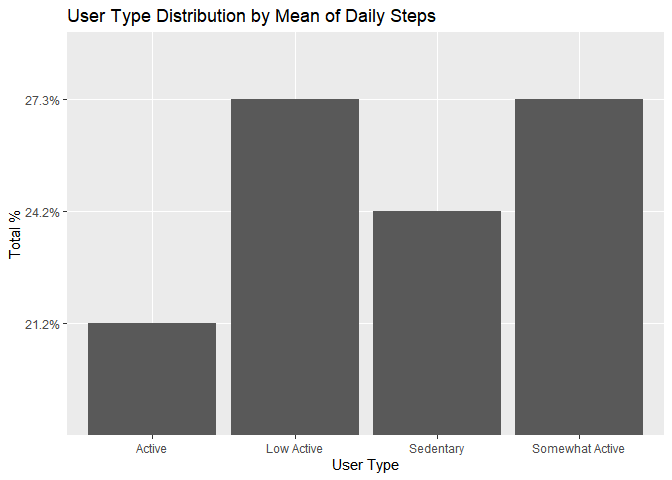
\includegraphics{GOOGLE-DATA-ANALYSIS-CASE-STUDY_files/figure-latex/unnamed-chunk-27-1.pdf}

From the graph, Low Active (27.3\%) and Somewhat Active(27.3\%) are
relatively distributed among the user.

\hypertarget{weight-log-info}{%
\paragraph{2. WEIGHT LOG INFO}\label{weight-log-info}}

\begin{Shaded}
\begin{Highlighting}[]
\CommentTok{\#Summary of weight\_log\_info}
\FunctionTok{summary}\NormalTok{(new\_weight\_log\_info)}
\end{Highlighting}
\end{Shaded}

\begin{verbatim}
##        Id                Date              WeightKg       WeightPounds  
##  Min.   :1.504e+09   Length:67          Min.   : 52.60   Min.   :116.0  
##  1st Qu.:6.962e+09   Class :character   1st Qu.: 61.40   1st Qu.:135.4  
##  Median :6.962e+09   Mode  :character   Median : 62.50   Median :137.8  
##  Mean   :7.009e+09                      Mean   : 72.04   Mean   :158.8  
##  3rd Qu.:8.878e+09                      3rd Qu.: 85.05   3rd Qu.:187.5  
##  Max.   :8.878e+09                      Max.   :133.50   Max.   :294.3  
##       BMI        IsManualReport         LogId              New_Date         
##  Min.   :21.45   Length:67          Min.   :1.460e+12   Min.   :2016-04-12  
##  1st Qu.:23.96   Class :character   1st Qu.:1.461e+12   1st Qu.:2016-04-19  
##  Median :24.39   Mode  :character   Median :1.462e+12   Median :2016-04-27  
##  Mean   :25.19                      Mean   :1.462e+12   Mean   :2016-04-26  
##  3rd Qu.:25.56                      3rd Qu.:1.462e+12   3rd Qu.:2016-05-04  
##  Max.   :47.54                      Max.   :1.463e+12   Max.   :2016-05-12  
##     Month             WeekDay         
##  Length:67          Length:67         
##  Class :character   Class :character  
##  Mode  :character   Mode  :character  
##                                       
##                                       
## 
\end{verbatim}

The average weightkg is 72.04kg Average BMI is 25.19

\hypertarget{daily-sleep}{%
\paragraph{3. DAILY SLEEP}\label{daily-sleep}}

\begin{Shaded}
\begin{Highlighting}[]
\CommentTok{\#Summary of daily\_sleep}
\FunctionTok{summary}\NormalTok{(new\_daily\_sleep)}
\end{Highlighting}
\end{Shaded}

\begin{verbatim}
##        Id              SleepDay         TotalSleepRecords TotalMinutesAsleep
##  Min.   :1.504e+09   Length:407         Min.   :1.00      Min.   : 58.0     
##  1st Qu.:3.977e+09   Class :character   1st Qu.:1.00      1st Qu.:361.0     
##  Median :4.703e+09   Mode  :character   Median :1.00      Median :432.0     
##  Mean   :4.989e+09                      Mean   :1.12      Mean   :418.9     
##  3rd Qu.:6.962e+09                      3rd Qu.:1.00      3rd Qu.:490.0     
##  Max.   :8.792e+09                      Max.   :3.00      Max.   :796.0     
##  TotalTimeInBed       Date               Month             Weekday         
##  Min.   : 61.0   Min.   :2016-04-12   Length:407         Length:407        
##  1st Qu.:404.5   1st Qu.:2016-04-19   Class :character   Class :character  
##  Median :463.0   Median :2016-04-27   Mode  :character   Mode  :character  
##  Mean   :458.3   Mean   :2016-04-26                                        
##  3rd Qu.:526.0   3rd Qu.:2016-05-04                                        
##  Max.   :961.0   Max.   :2016-05-12
\end{verbatim}

The mean total minutes asleep is 418.9 The average total time in bed is
458.3 minutes

\hypertarget{daily-steps}{%
\subparagraph{4. DAILY STEPS}\label{daily-steps}}

\begin{Shaded}
\begin{Highlighting}[]
\CommentTok{\#Summary of daily\_steps}
\FunctionTok{summary}\NormalTok{(daily\_steps)}
\end{Highlighting}
\end{Shaded}

\begin{verbatim}
##        Id            ActivityDay          StepTotal    
##  Min.   :1.504e+09   Length:940         Min.   :    0  
##  1st Qu.:2.320e+09   Class :character   1st Qu.: 3790  
##  Median :4.445e+09   Mode  :character   Median : 7406  
##  Mean   :4.855e+09                      Mean   : 7638  
##  3rd Qu.:6.962e+09                      3rd Qu.:10727  
##  Max.   :8.878e+09                      Max.   :36019
\end{verbatim}

The average steptotal is 7638 steps

\hypertarget{to-calculate-the-most-active-days-of-the-week}{%
\paragraph{To calculate the most active days of the
week}\label{to-calculate-the-most-active-days-of-the-week}}

\hypertarget{using-the-totalsteps-by-weekday}{%
\paragraph{using the totalsteps by
weekday}\label{using-the-totalsteps-by-weekday}}

\begin{Shaded}
\begin{Highlighting}[]
\CommentTok{\# 1. Order the day of the week}
\NormalTok{daily\_activity}\SpecialCharTok{$}\NormalTok{WeekDay }\OtherTok{\textless{}{-}} \FunctionTok{ordered}\NormalTok{(daily\_activity}\SpecialCharTok{$}\NormalTok{WeekDay,}\AttributeTok{levels=}\FunctionTok{c}\NormalTok{(}\StringTok{"Monday"}\NormalTok{,}\StringTok{"Tuesday"}\NormalTok{,}\StringTok{"Wednesday"}\NormalTok{,}\StringTok{"Thursday"}\NormalTok{,}\StringTok{"Friday"}\NormalTok{,}\StringTok{"Saturday"}\NormalTok{,}\StringTok{"Sunday"}\NormalTok{))}

\FunctionTok{ggplot}\NormalTok{(}\AttributeTok{data =}\NormalTok{ daily\_activity, }\FunctionTok{aes}\NormalTok{(}\AttributeTok{x=}\NormalTok{ WeekDay, }\AttributeTok{y =}\NormalTok{ TotalSteps))}\SpecialCharTok{+}
  \FunctionTok{geom\_col}\NormalTok{(}\AttributeTok{fill=}\StringTok{"purple"}\NormalTok{) }\SpecialCharTok{+} \FunctionTok{labs}\NormalTok{(}\AttributeTok{x=}\StringTok{"WeekDay"}\NormalTok{,}\AttributeTok{y=}\StringTok{"TotalSteps"}\NormalTok{,}\AttributeTok{title =} \StringTok{"Week Day by Total Steps"}\NormalTok{)}
\end{Highlighting}
\end{Shaded}

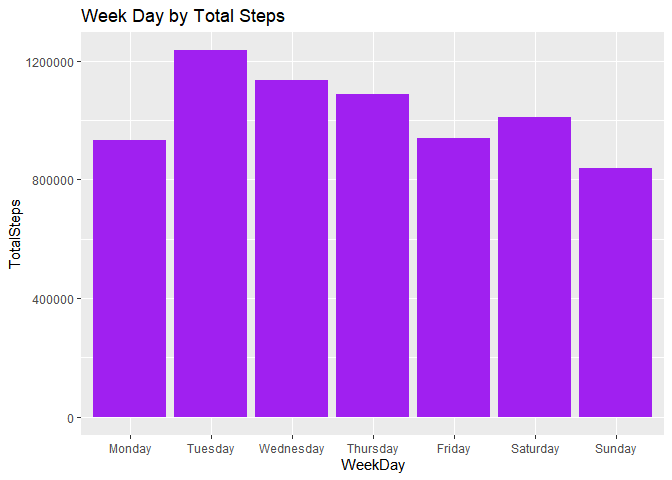
\includegraphics{GOOGLE-DATA-ANALYSIS-CASE-STUDY_files/figure-latex/unnamed-chunk-31-1.pdf}

User use FitBit fitness tracker application to track thier totalsteps
mostly Tuesday, Wednesday, Thursday.This behaviour can be term as a
result of users using the tracker to tack to track thierq daily
activities.

\hypertarget{using-the-veryactiveminutes-by-weekday}{%
\paragraph{using the VeryActiveMinutes by
weekday}\label{using-the-veryactiveminutes-by-weekday}}

\begin{Shaded}
\begin{Highlighting}[]
\CommentTok{\#2.  Order the day of the week}
\NormalTok{daily\_activity}\SpecialCharTok{$}\NormalTok{WeekDay }\OtherTok{\textless{}{-}} \FunctionTok{ordered}\NormalTok{(daily\_activity}\SpecialCharTok{$}\NormalTok{WeekDay,}\AttributeTok{levels=}\FunctionTok{c}\NormalTok{(}\StringTok{"Monday"}\NormalTok{,}\StringTok{"Tuesday"}\NormalTok{,}\StringTok{"Wednesday"}\NormalTok{,}\StringTok{"Thursday"}\NormalTok{,}\StringTok{"Friday"}\NormalTok{,}\StringTok{"Saturday"}\NormalTok{,}\StringTok{"Sunday"}\NormalTok{))}


\FunctionTok{ggplot}\NormalTok{(}\AttributeTok{data =}\NormalTok{ daily\_activity, }\FunctionTok{aes}\NormalTok{(}\AttributeTok{x=}\NormalTok{ WeekDay, }\AttributeTok{y =}\NormalTok{ VeryActiveMinutes))}\SpecialCharTok{+}
  \FunctionTok{geom\_col}\NormalTok{(}\AttributeTok{fill=}\StringTok{"blue"}\NormalTok{) }\SpecialCharTok{+} \FunctionTok{labs}\NormalTok{(}\AttributeTok{x=}\StringTok{"WeekDay"}\NormalTok{,}\AttributeTok{y=}\StringTok{"VeryActiveMinutes"}\NormalTok{,}\AttributeTok{title =} \StringTok{"Week Day by Very Active Minutes"}\NormalTok{)}
\end{Highlighting}
\end{Shaded}

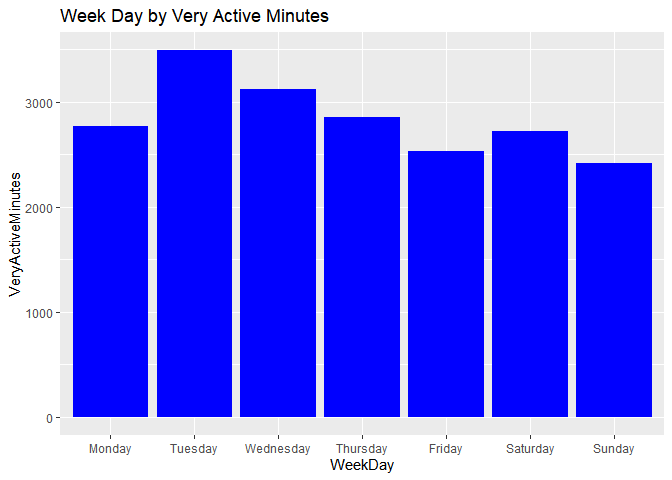
\includegraphics{GOOGLE-DATA-ANALYSIS-CASE-STUDY_files/figure-latex/unnamed-chunk-32-1.pdf}

\hypertarget{using-the-calories-by-weekday}{%
\paragraph{using the Calories by
weekday}\label{using-the-calories-by-weekday}}

\begin{Shaded}
\begin{Highlighting}[]
\CommentTok{\# 3. Order the day of the week}
\NormalTok{daily\_activity}\SpecialCharTok{$}\NormalTok{WeekDay }\OtherTok{\textless{}{-}} \FunctionTok{ordered}\NormalTok{(daily\_activity}\SpecialCharTok{$}\NormalTok{WeekDay,}\AttributeTok{levels=}\FunctionTok{c}\NormalTok{(}\StringTok{"Monday"}\NormalTok{,}\StringTok{"Tuesday"}\NormalTok{,}\StringTok{"Wednesday"}\NormalTok{,}\StringTok{"Thursday"}\NormalTok{,}\StringTok{"Friday"}\NormalTok{,}\StringTok{"Saturday"}\NormalTok{,}\StringTok{"Sunday"}\NormalTok{))}


\FunctionTok{ggplot}\NormalTok{(}\AttributeTok{data =}\NormalTok{ daily\_activity)}\SpecialCharTok{+} \FunctionTok{geom\_col}\NormalTok{(}\FunctionTok{aes}\NormalTok{(}\AttributeTok{x=}\NormalTok{ WeekDay, }\AttributeTok{y =}\NormalTok{ Calories),}\AttributeTok{fill=} \StringTok{"orange"}\NormalTok{)}\SpecialCharTok{+}
  \FunctionTok{labs}\NormalTok{(}\AttributeTok{x=}\StringTok{"WeekDay"}\NormalTok{,}\AttributeTok{y=}\StringTok{"Calories"}\NormalTok{,}\AttributeTok{title =} \StringTok{"Week Day by Calories"}\NormalTok{)}
\end{Highlighting}
\end{Shaded}

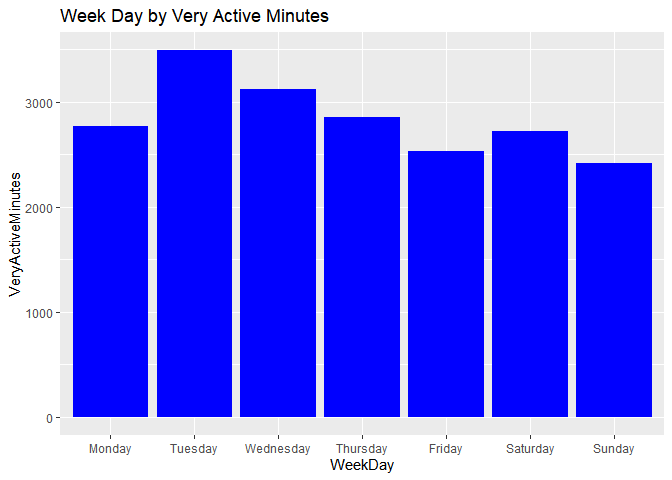
\includegraphics{GOOGLE-DATA-ANALYSIS-CASE-STUDY_files/figure-latex/unnamed-chunk-33-1.pdf}

User use FitBit fitness tracker application to track thier calories and
Tuesday, Wednesday , Thursday have the hightest caloires burned.

\hypertarget{for-daily-activity-relation-between-total-steps-and-sedentaryminutes}{%
\paragraph{1. for Daily activity (Relation between Total Steps and
SedentaryMinutes)}\label{for-daily-activity-relation-between-total-steps-and-sedentaryminutes}}

\begin{Shaded}
\begin{Highlighting}[]
\FunctionTok{ggplot}\NormalTok{ (}\AttributeTok{data=}\NormalTok{ daily\_activity, }\FunctionTok{aes}\NormalTok{(}\AttributeTok{x=}\NormalTok{TotalSteps, }\AttributeTok{y=}\NormalTok{SedentaryMinutes,}\AttributeTok{color=}\NormalTok{ Calories))}\SpecialCharTok{+}
  \FunctionTok{geom\_point}\NormalTok{()}\SpecialCharTok{+} \FunctionTok{labs}\NormalTok{(}\AttributeTok{x=}\StringTok{"Total Steps"}\NormalTok{,}\AttributeTok{y=}\StringTok{"Sedentary Minutes"}\NormalTok{,}\AttributeTok{title=}\StringTok{"Total Steps by Sedentary Minutes"}\NormalTok{)}
\end{Highlighting}
\end{Shaded}

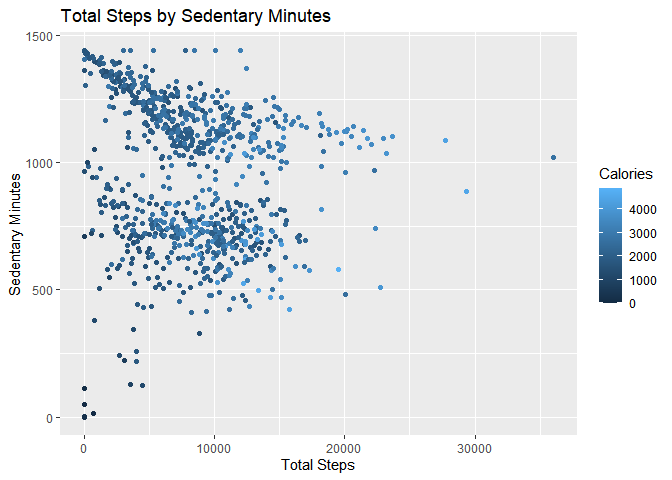
\includegraphics{GOOGLE-DATA-ANALYSIS-CASE-STUDY_files/figure-latex/unnamed-chunk-34-1.pdf}

From the scatter graph, there is a negative relationship between total
steps and sedentary miutes because people do not move when they are not
physically active

\hypertarget{for-daily-activity-to-find-if-there-is-a-relation-between-total-steps-by-calories-and-colour-of-the-line-can-be-controlled-using-colour-aesthetic}{%
\paragraph{2. for Daily activity (To find if there is a relation between
Total Steps by calories and colour of the line can be controlled using
colour
aesthetic}\label{for-daily-activity-to-find-if-there-is-a-relation-between-total-steps-by-calories-and-colour-of-the-line-can-be-controlled-using-colour-aesthetic}}

\begin{Shaded}
\begin{Highlighting}[]
\FunctionTok{ggplot}\NormalTok{(}\AttributeTok{data=}\NormalTok{daily\_activity, }\FunctionTok{aes}\NormalTok{(}\AttributeTok{x=}\NormalTok{TotalSteps, }\AttributeTok{y =}\NormalTok{ Calories))}\SpecialCharTok{+} \FunctionTok{geom\_point}\NormalTok{() }\SpecialCharTok{+} \FunctionTok{stat\_smooth}\NormalTok{(}\AttributeTok{method=}\NormalTok{lm, }\AttributeTok{fill=}\StringTok{"blue"}\NormalTok{, }\AttributeTok{colour=}\StringTok{"darkblue"}\NormalTok{, }\AttributeTok{size=}\DecValTok{1}\NormalTok{)}\SpecialCharTok{+}
  \FunctionTok{labs}\NormalTok{(}\AttributeTok{x=}\StringTok{"Total Steps"}\NormalTok{,}\AttributeTok{y=}\StringTok{"Calories"}\NormalTok{,}\AttributeTok{title=}\StringTok{"Total Steps by Calories"}\NormalTok{)}
\end{Highlighting}
\end{Shaded}

\begin{verbatim}
## `geom_smooth()` using formula 'y ~ x'
\end{verbatim}

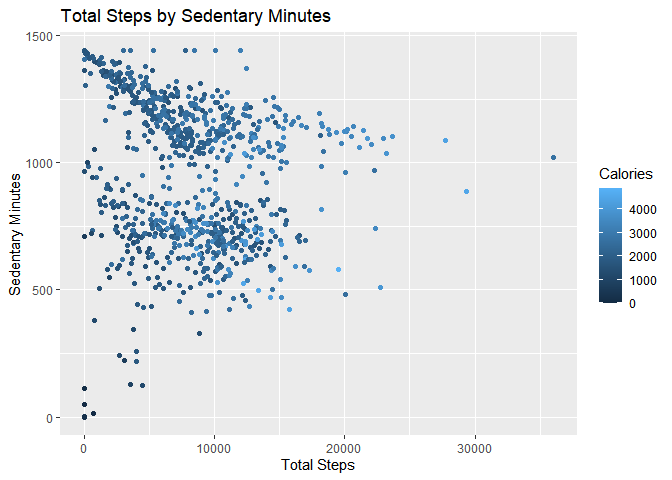
\includegraphics{GOOGLE-DATA-ANALYSIS-CASE-STUDY_files/figure-latex/unnamed-chunk-35-1.pdf}

From the plotted scatter graph, there is a positivecorrelation between
the totalsteps and calories people that took the most total steps burn
the most calories i.e the higher the steps the more calories user burn.

\hypertarget{to-find-if-there-is-a-relation-between-sleep-and-time-in-bed}{%
\paragraph{3. To find if there is a relation between sleep and time in
bed?}\label{to-find-if-there-is-a-relation-between-sleep-and-time-in-bed}}

\begin{Shaded}
\begin{Highlighting}[]
\FunctionTok{ggplot}\NormalTok{(}\AttributeTok{data=}\NormalTok{ new\_daily\_sleep, }\FunctionTok{aes}\NormalTok{(}\AttributeTok{x=}\NormalTok{TotalMinutesAsleep, }\AttributeTok{y=}\NormalTok{TotalTimeInBed)) }\SpecialCharTok{+} \FunctionTok{geom\_point}\NormalTok{() }\SpecialCharTok{+} \FunctionTok{stat\_smooth}\NormalTok{(}\AttributeTok{method =}\NormalTok{ lm,  }\AttributeTok{fill=}\StringTok{"blue"}\NormalTok{, }\AttributeTok{colour=}\StringTok{"darkblue"}\NormalTok{, }\AttributeTok{size=}\DecValTok{1}\NormalTok{)}\SpecialCharTok{+}
  \FunctionTok{labs}\NormalTok{(}\AttributeTok{x=}\StringTok{"Total Minutes Asleep"}\NormalTok{,}\AttributeTok{y=}\StringTok{"Total Time In Bed"}\NormalTok{,}\AttributeTok{title=}\StringTok{"Total Minutes Asleep by Total Time In Bed"}\NormalTok{)}
\end{Highlighting}
\end{Shaded}

\begin{verbatim}
## `geom_smooth()` using formula 'y ~ x'
\end{verbatim}

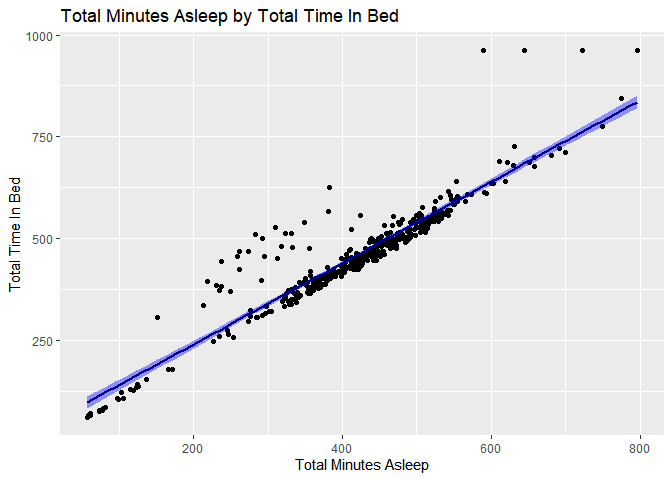
\includegraphics{GOOGLE-DATA-ANALYSIS-CASE-STUDY_files/figure-latex/unnamed-chunk-36-1.pdf}

From the scatter graph, we noticed a strong positive correlation between
TotalMinutesAsleep and TotalTimeInBed also we observed some outliers in
the middle and top of the scatter plot. we can say the outliers are the
people who spend lot of time in bed but did not actually sleep due to
different reasons. To improve the sleep hours, a beep on the bellet time
watch should be use to prepare user to sleep.

\hypertarget{to-find-if-there-is-relationship-between-active-minutes-and-calories}{%
\paragraph{4. To find if there is Relationship between active minutes
and
calories}\label{to-find-if-there-is-relationship-between-active-minutes-and-calories}}

\begin{Shaded}
\begin{Highlighting}[]
\FunctionTok{ggplot}\NormalTok{(}\AttributeTok{data=}\NormalTok{daily\_activity,}\FunctionTok{aes}\NormalTok{(}\AttributeTok{x =}\NormalTok{ VeryActiveMinutes, }\AttributeTok{y =}\NormalTok{ Calories, }\AttributeTok{color =}\NormalTok{ Calories)) }\SpecialCharTok{+} \FunctionTok{geom\_point}\NormalTok{() }\SpecialCharTok{+} \FunctionTok{stat\_smooth}\NormalTok{(}\AttributeTok{method =}\NormalTok{ lm,  }\AttributeTok{fill=}\StringTok{"orange"}\NormalTok{, }\AttributeTok{colour=}\StringTok{"darkorange"}\NormalTok{, }\AttributeTok{size=}\DecValTok{1}\NormalTok{)}\SpecialCharTok{+}
\FunctionTok{labs}\NormalTok{(}\AttributeTok{x=}\StringTok{"Very Active Minutes"}\NormalTok{,}\AttributeTok{y=}\StringTok{"Calories"}\NormalTok{,}\AttributeTok{title =} \StringTok{"Very Active Minutes by Calories Burned"}\NormalTok{)}
\end{Highlighting}
\end{Shaded}

\begin{verbatim}
## `geom_smooth()` using formula 'y ~ x'
\end{verbatim}

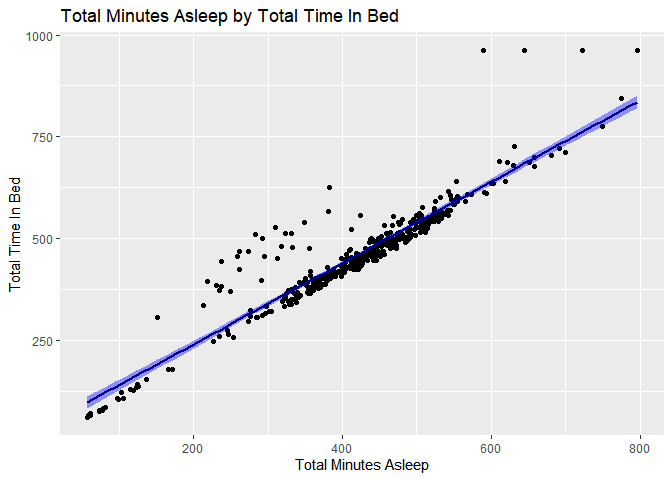
\includegraphics{GOOGLE-DATA-ANALYSIS-CASE-STUDY_files/figure-latex/unnamed-chunk-37-1.pdf}

From the graph, there is a strong correlation between very active
minutes and calories burned with some outliers at bottom left and top
left of the plot.

\hypertarget{to-plot-daily-sleep-per-week-day}{%
\paragraph{To plot daily sleep per week
day}\label{to-plot-daily-sleep-per-week-day}}

\begin{Shaded}
\begin{Highlighting}[]
\CommentTok{\# Order the day of the week}
\NormalTok{new\_daily\_sleep}\SpecialCharTok{$}\NormalTok{Weekday }\OtherTok{\textless{}{-}} \FunctionTok{ordered}\NormalTok{(new\_daily\_sleep}\SpecialCharTok{$}\NormalTok{Weekday,}\AttributeTok{levels=}\FunctionTok{c}\NormalTok{(}\StringTok{"Monday"}\NormalTok{,}\StringTok{"Tuesday"}\NormalTok{,}\StringTok{"Wednesday"}\NormalTok{,}\StringTok{"Thursday"}\NormalTok{,}\StringTok{"Friday"}\NormalTok{,}\StringTok{"Saturday"}\NormalTok{,}\StringTok{"Sunday"}\NormalTok{))}


\FunctionTok{ggplot}\NormalTok{(}\AttributeTok{data =}\NormalTok{ new\_daily\_sleep, }\FunctionTok{aes}\NormalTok{(}\AttributeTok{x=}\NormalTok{ Weekday, }\AttributeTok{y =}\NormalTok{ TotalMinutesAsleep))}\SpecialCharTok{+}
  \FunctionTok{geom\_col}\NormalTok{() }\SpecialCharTok{+} \FunctionTok{labs}\NormalTok{(}\AttributeTok{x=}\StringTok{"Weekday"}\NormalTok{,}\AttributeTok{y=}\StringTok{"Total Minutes Asleep"}\NormalTok{,}\AttributeTok{title =} \StringTok{"Total Minutes Asleep By Week Day"}\NormalTok{)}
\end{Highlighting}
\end{Shaded}

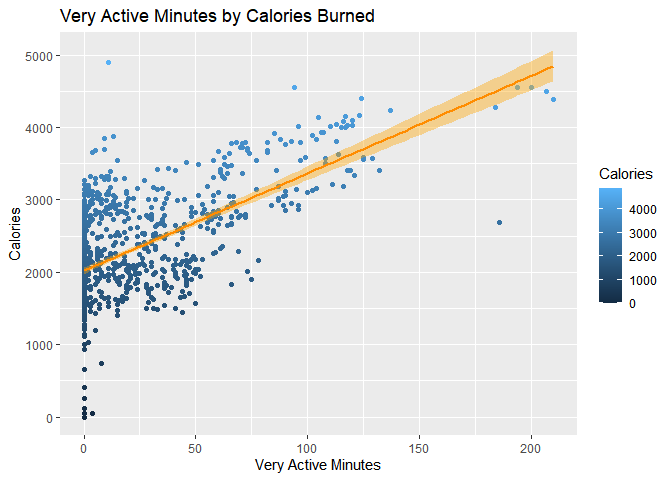
\includegraphics{GOOGLE-DATA-ANALYSIS-CASE-STUDY_files/figure-latex/unnamed-chunk-38-1.pdf}

User sleep most on Wednesday, and Tuesday while the least sleep day is
on Monday.

\hypertarget{to-analyze-the-relationship-of-weight-data-merge-dailyactivity-and-new-weight-log-info-dataframes}{%
\paragraph{To analyze the relationship of weight data, merge
dailyactivity and new weight log info
dataframes}\label{to-analyze-the-relationship-of-weight-data-merge-dailyactivity-and-new-weight-log-info-dataframes}}

\begin{Shaded}
\begin{Highlighting}[]
\NormalTok{weight\_daily\_activity }\OtherTok{\textless{}{-}} \FunctionTok{merge}\NormalTok{(daily\_activity,new\_weight\_log\_info, }\AttributeTok{by =} \StringTok{"Id"}\NormalTok{)}
\FunctionTok{head}\NormalTok{(weight\_daily\_activity)}
\end{Highlighting}
\end{Shaded}

\begin{verbatim}
##           Id ActivityDate TotalSteps TotalDistance TrackerDistance
## 1 1503960366    4/16/2016      12669          8.16            8.16
## 2 1503960366    4/16/2016      12669          8.16            8.16
## 3 1503960366    4/18/2016      13019          8.59            8.59
## 4 1503960366    4/18/2016      13019          8.59            8.59
## 5 1503960366    4/15/2016       9762          6.28            6.28
## 6 1503960366    4/15/2016       9762          6.28            6.28
##   LoggedActivitiesDistance VeryActiveDistance ModeratelyActiveDistance
## 1                        0               2.71                     0.41
## 2                        0               2.71                     0.41
## 3                        0               3.25                     0.64
## 4                        0               3.25                     0.64
## 5                        0               2.14                     1.26
## 6                        0               2.14                     1.26
##   LightActiveDistance SedentaryActiveDistance VeryActiveMinutes
## 1                5.04                       0                36
## 2                5.04                       0                36
## 3                4.71                       0                42
## 4                4.71                       0                42
## 5                2.83                       0                29
## 6                2.83                       0                29
##   FairlyActiveMinutes LightlyActiveMinutes SedentaryMinutes Calories     Date.x
## 1                  10                  221              773     1863 2016-04-16
## 2                  10                  221              773     1863 2016-04-16
## 3                  16                  233             1149     1921 2016-04-18
## 4                  16                  233             1149     1921 2016-04-18
## 5                  34                  209              726     1745 2016-04-15
## 6                  34                  209              726     1745 2016-04-15
##   Month.x WeekDay.x               Date.y WeightKg WeightPounds   BMI
## 1   April  Saturday 5/2/2016 11:59:59 PM     52.6     115.9631 22.65
## 2   April  Saturday 5/3/2016 11:59:59 PM     52.6     115.9631 22.65
## 3   April    Monday 5/2/2016 11:59:59 PM     52.6     115.9631 22.65
## 4   April    Monday 5/3/2016 11:59:59 PM     52.6     115.9631 22.65
## 5   April    Friday 5/2/2016 11:59:59 PM     52.6     115.9631 22.65
## 6   April    Friday 5/3/2016 11:59:59 PM     52.6     115.9631 22.65
##   IsManualReport        LogId   New_Date Month.y WeekDay.y
## 1           True 1.462234e+12 2016-05-02     May    Monday
## 2           True 1.462320e+12 2016-05-03     May   Tuesday
## 3           True 1.462234e+12 2016-05-02     May    Monday
## 4           True 1.462320e+12 2016-05-03     May   Tuesday
## 5           True 1.462234e+12 2016-05-02     May    Monday
## 6           True 1.462320e+12 2016-05-03     May   Tuesday
\end{verbatim}

\begin{Shaded}
\begin{Highlighting}[]
\FunctionTok{summary}\NormalTok{(weight\_daily\_activity)}
\end{Highlighting}
\end{Shaded}

\begin{verbatim}
##        Id            ActivityDate         TotalSteps    TotalDistance   
##  Min.   :1.504e+09   Length:2076        Min.   :    0   Min.   : 0.000  
##  1st Qu.:6.962e+09   Class :character   1st Qu.: 7948   1st Qu.: 5.367  
##  Median :6.962e+09   Mode  :character   Median :10762   Median : 7.410  
##  Mean   :7.010e+09                      Mean   :11648   Mean   : 8.696  
##  3rd Qu.:8.878e+09                      3rd Qu.:13928   3rd Qu.: 9.550  
##  Max.   :8.878e+09                      Max.   :29326   Max.   :26.720  
##                                                                         
##  TrackerDistance  LoggedActivitiesDistance VeryActiveDistance
##  Min.   : 0.000   Min.   :0.000            Min.   : 0.0000   
##  1st Qu.: 5.367   1st Qu.:0.000            1st Qu.: 0.1375   
##  Median : 7.410   Median :0.000            Median : 1.7400   
##  Mean   : 8.666   Mean   :0.145            Mean   : 3.3042   
##  3rd Qu.: 9.080   3rd Qu.:0.000            3rd Qu.: 3.9000   
##  Max.   :26.720   Max.   :4.082            Max.   :21.6600   
##                                                              
##  ModeratelyActiveDistance LightActiveDistance SedentaryActiveDistance
##  Min.   :0.000            Min.   : 0.000      Min.   :0.000000       
##  1st Qu.:0.080            1st Qu.: 3.610      1st Qu.:0.000000       
##  Median :0.410            Median : 4.660      Median :0.000000       
##  Mean   :0.659            Mean   : 4.701      Mean   :0.005039       
##  3rd Qu.:1.070            3rd Qu.: 5.890      3rd Qu.:0.000000       
##  Max.   :2.390            Max.   :10.710      Max.   :0.110000       
##                                                                      
##  VeryActiveMinutes FairlyActiveMinutes LightlyActiveMinutes SedentaryMinutes
##  Min.   :  0.00    Min.   : 0.00       Min.   :  0.0        Min.   :   0.0  
##  1st Qu.:  7.00    1st Qu.: 4.00       1st Qu.:210.8        1st Qu.: 680.0  
##  Median : 29.00    Median :12.00       Median :235.5        Median : 837.0  
##  Mean   : 37.63    Mean   :14.45       Mean   :240.8        Mean   : 887.8  
##  3rd Qu.: 61.00    3rd Qu.:22.00       3rd Qu.:288.0        3rd Qu.:1122.2  
##  Max.   :210.00    Max.   :74.00       Max.   :448.0        Max.   :1440.0  
##                                                                             
##     Calories        Date.x             Month.x              WeekDay.x  
##  Min.   :   0   Min.   :2016-04-12   Length:2076        Monday   :268  
##  1st Qu.:1994   1st Qu.:2016-04-19   Class :character   Tuesday  :335  
##  Median :2174   Median :2016-04-27   Mode  :character   Wednesday:335  
##  Mean   :2519   Mean   :2016-04-26                      Thursday :334  
##  3rd Qu.:3060   3rd Qu.:2016-05-05                      Friday   :268  
##  Max.   :4552   Max.   :2016-05-12                      Saturday :268  
##                                                         Sunday   :268  
##     Date.y             WeightKg       WeightPounds        BMI       
##  Length:2076        Min.   : 52.60   Min.   :116.0   Min.   :21.45  
##  Class :character   1st Qu.: 61.40   1st Qu.:135.4   1st Qu.:23.96  
##  Mode  :character   Median : 62.50   Median :137.8   Median :24.39  
##                     Mean   : 72.03   Mean   :158.8   Mean   :25.18  
##                     3rd Qu.: 85.10   3rd Qu.:187.6   3rd Qu.:25.56  
##                     Max.   :133.50   Max.   :294.3   Max.   :47.54  
##                                                                     
##  IsManualReport         LogId              New_Date            Month.y         
##  Length:2076        Min.   :1.460e+12   Min.   :2016-04-12   Length:2076       
##  Class :character   1st Qu.:1.461e+12   1st Qu.:2016-04-19   Class :character  
##  Mode  :character   Median :1.462e+12   Median :2016-04-27   Mode  :character  
##                     Mean   :1.462e+12   Mean   :2016-04-26                     
##                     3rd Qu.:1.462e+12   3rd Qu.:2016-05-04                     
##                     Max.   :1.463e+12   Max.   :2016-05-12                     
##                                                                                
##   WeekDay.y        
##  Length:2076       
##  Class :character  
##  Mode  :character  
##                    
##                    
##                    
## 
\end{verbatim}

\hypertarget{to-plot-the-relationship-between-veryactiveminutes-and-weightin-kg}{%
\paragraph{To plot the relationship between veryactiveminutes and
weightin
kg}\label{to-plot-the-relationship-between-veryactiveminutes-and-weightin-kg}}

\begin{Shaded}
\begin{Highlighting}[]
\FunctionTok{ggplot}\NormalTok{(}\AttributeTok{data=}\NormalTok{weight\_daily\_activity) }\SpecialCharTok{+} \FunctionTok{geom\_violin}\NormalTok{(}\AttributeTok{mapping=}\FunctionTok{aes}\NormalTok{(}\AttributeTok{x=}\NormalTok{VeryActiveMinutes, }\AttributeTok{y=}\NormalTok{WeightKg), }\AttributeTok{fill =} \StringTok{"blue"}\NormalTok{) }\SpecialCharTok{+}
\FunctionTok{labs}\NormalTok{(}\AttributeTok{title=}\StringTok{"Violin plot"}\NormalTok{, }\AttributeTok{subtitle=}\StringTok{"User Weight by Very Active Minutes"}\NormalTok{, }\AttributeTok{x=}\StringTok{"Very Active Minutes"}\NormalTok{, }\AttributeTok{y=}\StringTok{"Weight in Kg"}\NormalTok{)}
\end{Highlighting}
\end{Shaded}

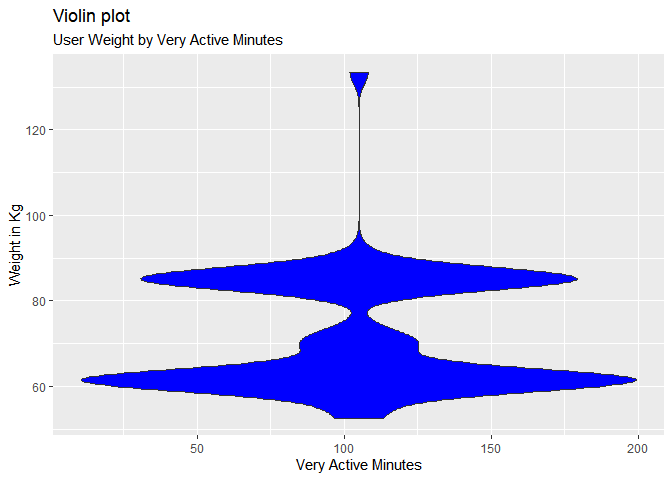
\includegraphics{GOOGLE-DATA-ANALYSIS-CASE-STUDY_files/figure-latex/unnamed-chunk-40-1.pdf}

From the violin plot, the median weight is 63.

Most users have a weight that is between 61 and 85, but some users have
weight that are low as 53 and as high as 134. From the plot we can see
outlier weight to be 134.

\hypertarget{act-phase-conclusion-and-recommendation}{%
\paragraph{\texorpdfstring{\textbf{ACT PHASE (CONCLUSION AND
RECOMMENDATION)}}{ACT PHASE (CONCLUSION AND RECOMMENDATION)}}\label{act-phase-conclusion-and-recommendation}}

From the analysis carried out and using the business questions:

\begin{itemize}
\item
  The average total steps per day is 7638 which is below the 10,000
  recommended steps per day which is termed the gold standards for
  adults. Therefore, the app should track users who do not meet the
  10,000 recommended steps per day and send a reminder to to encourage
  them
\item
  People tend to be more active on on Tuesday, Wednesday and Thursday so
  they tend to use their app on week days maybe because they spend more
  time outside compare to weekends
\item
  Most users weight in Kg is between 61 - 85. Since bellabeat focus is
  on young and adult women empowerment and the data lack information on
  women Gender and Age therefore, there is need for more data on young
  and adult female gender, and age in order to meet bellabeat mission.
\item
  Bellabeat marketing team can encourage users by educating them the
  benefits of the fitness, recommend the types of exercises users can
  partake in, calories intake and burn rate information on bellabeat
  application.
\item
  The Bellebeat application should always send reminder during weekends
  to encourage users to exercise regularly.
\item
  The Bellabeat app should create a reward system such that users who
  meet their daily steps goals would earn points which can be converted
  to discount for bellabeat membership at the end of every year
\end{itemize}

\end{document}
